\subsection{Non-Uniform Rational B-Spline (NURBS)}
\label{lr_sec:NURBS}
\paragraph{}
In the proposed approach, the geometry and the unknown fields are represented by non-uniform rational B-splines (NURBS).
In this section, we give a brief overview of NURBS.
For more detailed description and implementation aspects, interested readers can refer to \citep{Pie1997,NGUYEN201589}.
\paragraph{}
% basis function
NURBS are the superset of B-spline functions.
B-spline is short for basis spline and is a generalization of Bézier curves.
A spline function is a piecewise polynomial function of degree $p$ and the points of intersection of such functions are called knots.
The number of knots must be equal to or greater than $p + 1$.
One of the salient features of spline functions is that the functions are continuous at the knots, however, the continuity of the functions can be altered by repeating the knots.
The B-spline functions are parametric functions of the form $F(\eta)$ in which the parameter $\eta$ lies in the parametric space.
The key ingredients in the construction of B-spline functions are: the knot vector (a non decreasing sequence of parameter values, $\eta_i \leq \eta_{i+1}$ , $i = 0,1,\dots,m -1$) and the degree of the curve p. The $i$th B-spline basis function of degree $p$, denoted by $_{i,p}$ is defined as \citep{Pie1997}:
\begin{equation}
    \begin{aligned}
        N_{i,0}(\eta) &=
            \begin{cases}
                1   & \text{if } \eta_i \leq \eta \leq \eta_{i+1}    \\
                0   & \text{else}
            \end{cases}\\
        N_{i,p}(\eta) &= 
            \frac{\eta - \eta_i}{\eta_{i+p}-\eta_i}     N_{i,p-1}(\eta) - 
            \frac{\eta_{i+p+1}-\eta}{\eta_{i+p+1} - \eta_{i+1}}     N_{i+1,p-1}(\eta)
    \end{aligned}
    \label{lr_nurbs_basis}
\end{equation}

The first derivative of the B-spline basis function can be computed recursively from lower order basis functions as:
\begin{equation}
    \frac{d}{d\eta} N_{i,p}(\eta) =
        \frac{p}{\eta_{i+p} - \eta_i} N_{i,p-1}(\eta) -
        \frac{p}{\eta_{i+p+1} - \eta_{i+1}} N_{i+1,p-1}(\eta)
\end{equation}

\paragraph{}
% basis properties
The B-spline basis functions has the following properties:
\begin{enumerate}
    \item Non-negativity
    \item Partition of unity, $\sum_i N_{i,p}=1$
    \item Interpolatory at the end points. The last point requires special treatment when imposing non-homogeneous Dirichlet boundary conditions [58].
\end{enumerate}


\paragraph{}
% curves
Moreover, the spline function has limited support.
Given $n + 1$ control points $(P_0 ,P_1,\dots,P_n )$ and a knot vector 
    $\Xi$ = $\left\{
        \eta_0 ,\eta_1 ,\dots,\eta_m 
    \right\}$, the piecewise polynomial B-spline curve of degree p is defined as:
\begin{equation}
    C(\eta) = \sum_{i=0}^n P_i N_{i,p} (\eta)
\end{equation}

where $P_i$ are the control points.
A B-spline curve has the following information: $n+1$ control points, $m+1$ knots and a degree $p$.
It is noted that $n$,$m$ and $p$ must satisfy $m = n + p + 1$.
The B-spline functions also provide a variety of refinement algorithms, which are essential when employing B-spline functions to discretize the unknown fields.
The analogous $h$ and $p$ refinement can be done by the process of `knot insertion' and `order elevation'.
Another unique feature of the B-spline basis function is that, it is possible to combine the knot insertion and the degree elevation, commonly referred to as ‘k-refinement’ in the literature \citep{Hug2005b}.
Here we briefly discuss the knot insertion and the degree elevation.
For more details, interested readers are referred to \citep{Pie1997,Hug2005b} and references therein.


\subsubsection{Knot insertion}
\label{lr_sec:nurbs_knot_ins}
\paragraph{}
Consider a B-spline basis functions defined on 
$\Xi = \left\{
    \eta_0 ,\eta_1,\dots,\eta_m 
    \right\}$,
let $\overline{\eta} \in [\eta_k ,\eta_{k+1} )$, and insert $\overline{\eta}$ into $\Xi$ to form a new knot vector 
$\overline{\Xi} = \left\{
    \eta_0 ,\dots, \overline{\eta}_k = \eta_k , 
    \overline{\eta}_{k+1} = \overline{\eta}, 
    \overline{\eta}_{k+2} = \overline{\eta}_{k+1} ,
    \dots,\eta_{m+1} = \eta_m
    \right\}$.
Simultaneously, the size of the control points is increased by one. Thus $C(\eta)$ has a representation on $\overline{\Xi}$ of the form
\begin{equation}
    \mathbf{C}(\eta) = \sum_{i=0}^{n+1}
                        \overline{N}_{i,p} (\eta)
                        \mathbf{Q}_i
\end{equation}
Where $\mathbf{Q}_i$ is:
\begin{equation}
    \mathbf{Q}_i = \alpha_i \mathbf{P}_i +
                    (1-\alpha_i) \mathbf{P}_{i-1}
\end{equation}
where
\begin{equation}
    \alpha_i =  \begin{cases}
                    1       & i \leq k-p \\
                    \frac{ \overline{\eta} -\eta_i }{ \eta_{i+p} - \eta_i } & k-p \leq i \leq k \\
                    0 & i \geq k+1                          
                \end{cases}
\end{equation}


\subsubsection{Order elevation}
\label{lr_sec:nurbs_order_ele}
Let $
\mathbf{C}(\eta) =  \sum_{i=0}^n
                    N_{i,p}(\eta)
                    \mathbf{P}_i
$
be a $p$th-degree B-spline curve on the knot vector $\Xi$.
As a piecewise polynomial curve with $p+1$ order, $\mathbf{C}(\eta)$ is expected to be expressed in higher order basis functions.
In other words, another set of control points $Q_i$ and knot vector $\Xi$ should exists such that
\begin{equation}
    \mathbf{C}(\eta) =  \sum_{i=0}^{\overline{n}}
                        N_{i, p+1}(\eta)
                        \mathbf{Q}_i
\end{equation}
The procedure to elevate the order of a B-spline is listed as follows \citep{Pie1997}:
\begin{enumerate}
    \item Extract each Bézier segment from the curve
    \item Elevate the order of each Bézier segment
    \item Remove unnecessary knots separating the ($i-1$)th and $i$th segments
\end{enumerate}
When elevating a $p$th Bézier curve, a new set of control points can be determined from:
\begin{equation}
    \mathbf{Q}_i =  (1-\alpha_i) \mathbf{P}_i +
                    \alpha_i \mathbf{P}_{i-1}
\end{equation}
where $\alpha_i=\frac{i}{p+i}$, $i=0$, $\dots$, $p+1$.
Fig.~\ref{lr_fig:nurbs_knotins} and Fig.~\ref{lr_fig:nurbs_orderele} show an example of basis function when performing a knot insertion and order elevation, respectively.

\begin{figure}[h!]
    \centering
    % This file was created by matlab2tikz v0.4.6 running on MATLAB 8.0.
% Copyright (c) 2008--2014, Nico Schlömer <nico.schloemer@gmail.com>
% All rights reserved.
% Minimal pgfplots version: 1.3
% 
% The latest updates can be retrieved from
%   http://www.mathworks.com/matlabcentral/fileexchange/22022-matlab2tikz
% where you can also make suggestions and rate matlab2tikz.
% 
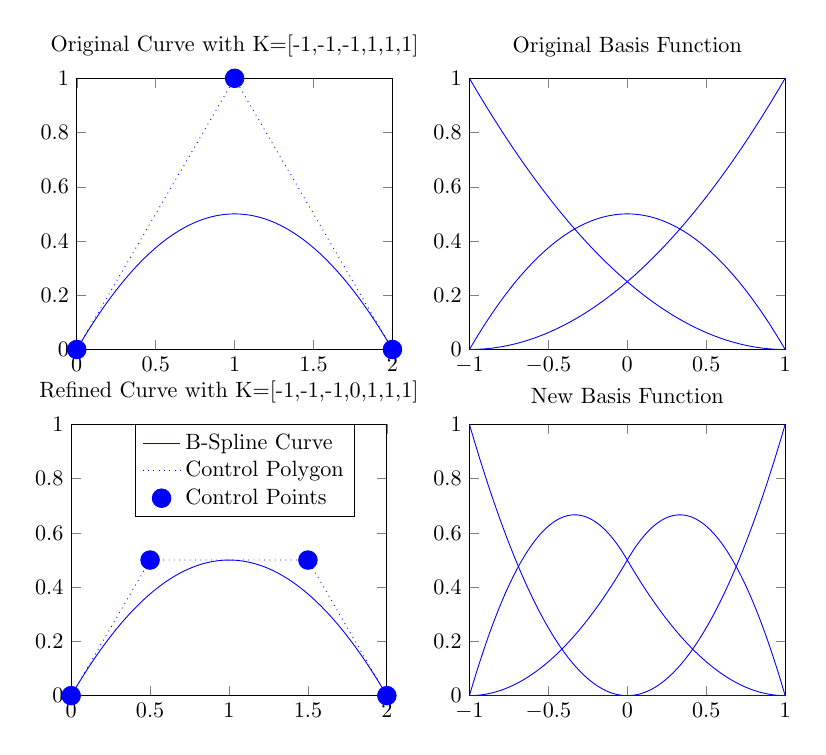
\begin{tikzpicture}[scale=0.8]

\begin{axis}[%
width=1.97309422348485in,
height=1.69505450581395in,
scale only axis,
xmin=0,
xmax=2,
ymin=0,
ymax=1,
name=plot1,
title={Original Curve with K=[-1,-1,-1,1,1,1]}
]
\addplot [color=blue,solid,forget plot]
  table[row sep=crcr]{
0	0	\\
0.0100502512562815	0.00999974748112426	\\
0.0201005025125628	0.019898487411934	\\
0.0301507537688442	0.0296962197924295	\\
0.0402010050251256	0.0393929446226105	\\
0.050251256281407	0.0489886619024772	\\
0.0603015075376885	0.0584833716320295	\\
0.0703517587939698	0.0678770738112674	\\
0.0804020100502513	0.0771697684401909	\\
0.0904522613065326	0.0863614555188	\\
0.100502512562814	0.0954521350470948	\\
0.110552763819096	0.104441807025075	\\
0.120603015075377	0.113330471452741	\\
0.130653266331658	0.122118128330093	\\
0.14070351758794	0.13080477765713	\\
0.150753768844221	0.139390419433853	\\
0.160804020100503	0.147875053660261	\\
0.170854271356784	0.156258680336355	\\
0.180904522613065	0.164541299462135	\\
0.190954773869347	0.1727229110376	\\
0.201005025125628	0.180803515062751	\\
0.21105527638191	0.188783111537587	\\
0.221105527638191	0.19666170046211	\\
0.231155778894472	0.204439281836317	\\
0.241206030150754	0.212115855660211	\\
0.251256281407035	0.21969142193379	\\
0.261306532663317	0.227165980657054	\\
0.271356783919598	0.234539531830004	\\
0.281407035175879	0.24181207545264	\\
0.291457286432161	0.248983611524961	\\
0.301507537688442	0.256054140046968	\\
0.311557788944724	0.263023661018661	\\
0.321608040201005	0.269892174440039	\\
0.331658291457286	0.276659680311103	\\
0.341708542713568	0.283326178631853	\\
0.351758793969849	0.289891669402288	\\
0.361809045226131	0.296356152622409	\\
0.371859296482412	0.302719628292215	\\
0.381909547738693	0.308982096411707	\\
0.391959798994975	0.315143556980884	\\
0.402010050251256	0.321204009999747	\\
0.412060301507538	0.327163455468296	\\
0.422110552763819	0.333021893386531	\\
0.4321608040201	0.338779323754451	\\
0.442211055276382	0.344435746572056	\\
0.452261306532663	0.349991161839347	\\
0.462311557788945	0.355445569556324	\\
0.472361809045226	0.360798969722987	\\
0.482412060301508	0.366051362339335	\\
0.492462311557789	0.371202747405369	\\
0.50251256281407	0.376253124921088	\\
0.512562814070352	0.381202494886493	\\
0.522613065326633	0.386050857301583	\\
0.532663316582915	0.390798212166359	\\
0.542713567839196	0.395444559480821	\\
0.552763819095477	0.399989899244969	\\
0.562814070351759	0.404434231458802	\\
0.57286432160804	0.40877755612232	\\
0.582914572864322	0.413019873235524	\\
0.592964824120603	0.417161182798414	\\
0.603015075376884	0.42120148481099	\\
0.613065326633166	0.425140779273251	\\
0.623115577889447	0.428979066185197	\\
0.633165829145729	0.43271634554683	\\
0.64321608040201	0.436352617358148	\\
0.653266331658292	0.439887881619151	\\
0.663316582914573	0.44332213832984	\\
0.673366834170854	0.446655387490215	\\
0.683417085427136	0.449887629100275	\\
0.693467336683417	0.453018863160021	\\
0.703517587939699	0.456049089669453	\\
0.71356783919598	0.45897830862857	\\
0.723618090452261	0.461806520037373	\\
0.733668341708543	0.464533723895861	\\
0.743718592964824	0.467159920204035	\\
0.753768844221106	0.469685108961895	\\
0.763819095477387	0.47210929016944	\\
0.773869346733668	0.474432463826671	\\
0.78391959798995	0.476654629933588	\\
0.793969849246231	0.47877578849019	\\
0.804020100502513	0.480795939496477	\\
0.814070351758794	0.482715082952451	\\
0.824120603015075	0.48453321885811	\\
0.834170854271357	0.486250347213454	\\
0.844221105527638	0.487866468018484	\\
0.85427135678392	0.4893815812732	\\
0.864321608040201	0.490795686977602	\\
0.874371859296482	0.492108785131689	\\
0.884422110552764	0.493320875735461	\\
0.894472361809045	0.494431958788919	\\
0.904522613065327	0.495442034292063	\\
0.914572864321608	0.496351102244893	\\
0.924623115577889	0.497159162647408	\\
0.934673366834171	0.497866215499609	\\
0.944723618090452	0.498472260801495	\\
0.954773869346734	0.498977298553067	\\
0.964824120603015	0.499381328754324	\\
0.974874371859296	0.499684351405268	\\
0.984924623115578	0.499886366505896	\\
0.994974874371859	0.499987374056211	\\
1.00502512562814	0.499987374056211	\\
1.01507537688442	0.499886366505896	\\
1.0251256281407	0.499684351405268	\\
1.03517587939699	0.499381328754324	\\
1.04522613065327	0.498977298553067	\\
1.05527638190955	0.498472260801495	\\
1.06532663316583	0.497866215499609	\\
1.07537688442211	0.497159162647408	\\
1.08542713567839	0.496351102244893	\\
1.09547738693467	0.495442034292063	\\
1.10552763819095	0.494431958788919	\\
1.11557788944724	0.493320875735461	\\
1.12562814070352	0.492108785131689	\\
1.1356783919598	0.490795686977602	\\
1.14572864321608	0.4893815812732	\\
1.15577889447236	0.487866468018484	\\
1.16582914572864	0.486250347213454	\\
1.17587939698492	0.48453321885811	\\
1.18592964824121	0.482715082952451	\\
1.19597989949749	0.480795939496477	\\
1.20603015075377	0.47877578849019	\\
1.21608040201005	0.476654629933588	\\
1.22613065326633	0.474432463826671	\\
1.23618090452261	0.47210929016944	\\
1.24623115577889	0.469685108961895	\\
1.25628140703518	0.467159920204035	\\
1.26633165829146	0.464533723895861	\\
1.27638190954774	0.461806520037373	\\
1.28643216080402	0.45897830862857	\\
1.2964824120603	0.456049089669453	\\
1.30653266331658	0.453018863160021	\\
1.31658291457286	0.449887629100275	\\
1.32663316582915	0.446655387490215	\\
1.33668341708543	0.44332213832984	\\
1.34673366834171	0.439887881619151	\\
1.35678391959799	0.436352617358148	\\
1.36683417085427	0.43271634554683	\\
1.37688442211055	0.428979066185197	\\
1.38693467336683	0.425140779273251	\\
1.39698492462312	0.42120148481099	\\
1.4070351758794	0.417161182798414	\\
1.41708542713568	0.413019873235524	\\
1.42713567839196	0.40877755612232	\\
1.43718592964824	0.404434231458802	\\
1.44723618090452	0.399989899244969	\\
1.4572864321608	0.395444559480821	\\
1.46733668341709	0.390798212166359	\\
1.47738693467337	0.386050857301583	\\
1.48743718592965	0.381202494886493	\\
1.49748743718593	0.376253124921088	\\
1.50753768844221	0.371202747405369	\\
1.51758793969849	0.366051362339335	\\
1.52763819095477	0.360798969722987	\\
1.53768844221106	0.355445569556324	\\
1.54773869346734	0.349991161839347	\\
1.55778894472362	0.344435746572056	\\
1.5678391959799	0.338779323754451	\\
1.57788944723618	0.333021893386531	\\
1.58793969849246	0.327163455468296	\\
1.59798994974874	0.321204009999747	\\
1.60804020100503	0.315143556980884	\\
1.61809045226131	0.308982096411707	\\
1.62814070351759	0.302719628292215	\\
1.63819095477387	0.296356152622409	\\
1.64824120603015	0.289891669402288	\\
1.65829145728643	0.283326178631853	\\
1.66834170854271	0.276659680311103	\\
1.67839195979899	0.269892174440039	\\
1.68844221105528	0.263023661018661	\\
1.69849246231156	0.256054140046968	\\
1.70854271356784	0.248983611524961	\\
1.71859296482412	0.24181207545264	\\
1.7286432160804	0.234539531830004	\\
1.73869346733668	0.227165980657054	\\
1.74874371859296	0.21969142193379	\\
1.75879396984925	0.212115855660211	\\
1.76884422110553	0.204439281836317	\\
1.77889447236181	0.19666170046211	\\
1.78894472361809	0.188783111537587	\\
1.79899497487437	0.180803515062751	\\
1.80904522613065	0.1727229110376	\\
1.81909547738693	0.164541299462135	\\
1.82914572864322	0.156258680336355	\\
1.8391959798995	0.147875053660261	\\
1.84924623115578	0.139390419433853	\\
1.85929648241206	0.13080477765713	\\
1.86934673366834	0.122118128330093	\\
1.87939698492462	0.113330471452741	\\
1.8894472361809	0.104441807025075	\\
1.89949748743719	0.0954521350470948	\\
1.90954773869347	0.0863614555188	\\
1.91959798994975	0.0771697684401908	\\
1.92964824120603	0.0678770738112675	\\
1.93969849246231	0.0584833716320295	\\
1.94974874371859	0.0489886619024772	\\
1.95979899497487	0.0393929446226105	\\
1.96984924623116	0.0296962197924294	\\
1.97989949748744	0.0198984874119341	\\
1.98994974874372	0.00999974748112426	\\
2	0	\\
};
\addplot [color=blue,dotted,forget plot]
  table[row sep=crcr]{
0	0	\\
1	1	\\
2	0	\\
};
\addplot [color=blue,mark size=4.2pt,only marks,mark=*,mark options={solid},forget plot]
  table[row sep=crcr]{
0	0	\\
1	1	\\
2	0	\\
};
\end{axis}

\begin{axis}[%
width=1.97309422348485in,
height=1.69505450581395in,
scale only axis,
xmin=-1,
xmax=1,
ymin=0,
ymax=1,
name=plot2,
at=(plot1.right of south east),
anchor=left of south west,
title={Original Basis Function}
]
\addplot [color=blue,solid,forget plot]
  table[row sep=crcr]{
-1	1	\\
-0.989949748743719	0.989975000631297	\\
-0.979899497487437	0.980000505037751	\\
-0.969849246231156	0.970076513219363	\\
-0.959798994974874	0.960203025176132	\\
-0.949748743718593	0.950380040908058	\\
-0.939698492462312	0.940607560415141	\\
-0.92964824120603	0.930885583697381	\\
-0.919597989949749	0.921214110754779	\\
-0.909547738693467	0.911593141587334	\\
-0.899497487437186	0.902022676195046	\\
-0.889447236180904	0.892502714577915	\\
-0.879396984924623	0.883033256735941	\\
-0.869346733668342	0.873614302669125	\\
-0.85929648241206	0.864245852377465	\\
-0.849246231155779	0.854927905860963	\\
-0.839195979899497	0.845660463119618	\\
-0.829145728643216	0.83644352415343	\\
-0.819095477386935	0.8272770889624	\\
-0.809045226130653	0.818161157546527	\\
-0.798994974874372	0.80909572990581	\\
-0.78894472361809	0.800080806040251	\\
-0.778894472361809	0.79111638594985	\\
-0.768844221105528	0.782202469634605	\\
-0.758793969849246	0.773339057094518	\\
-0.748743718592965	0.764526148329588	\\
-0.738693467336683	0.755763743339815	\\
-0.728643216080402	0.747051842125199	\\
-0.718592964824121	0.73839044468574	\\
-0.708542713567839	0.729779551021439	\\
-0.698492462311558	0.721219161132295	\\
-0.688442211055276	0.712709275018308	\\
-0.678391959798995	0.704249892679478	\\
-0.668341708542714	0.695841014115805	\\
-0.658291457286432	0.68748263932729	\\
-0.648241206030151	0.679174768313932	\\
-0.638190954773869	0.67091740107573	\\
-0.628140703517588	0.662710537612687	\\
-0.618090452261307	0.6545541779248	\\
-0.608040201005025	0.64644832201207	\\
-0.597989949748744	0.638392969874498	\\
-0.587939698492462	0.630388121512083	\\
-0.577889447236181	0.622433776924825	\\
-0.5678391959799	0.614529936112725	\\
-0.557788944723618	0.606676599075781	\\
-0.547738693467337	0.598873765813995	\\
-0.537688442211055	0.591121436327365	\\
-0.527638190954774	0.583419610615894	\\
-0.517587939698492	0.575768288679579	\\
-0.507537688442211	0.568167470518421	\\
-0.49748743718593	0.560617156132421	\\
-0.487437185929648	0.553117345521578	\\
-0.477386934673367	0.545668038685892	\\
-0.467336683417085	0.538269235625363	\\
-0.457286432160804	0.530920936339991	\\
-0.447236180904523	0.523623140829777	\\
-0.437185929648241	0.51637584909472	\\
-0.42713567839196	0.50917906113482	\\
-0.417085427135678	0.502032776950077	\\
-0.407035175879397	0.494936996540491	\\
-0.396984924623116	0.487891719906063	\\
-0.386934673366834	0.480896947046792	\\
-0.376884422110553	0.473952677962678	\\
-0.366834170854271	0.467058912653721	\\
-0.35678391959799	0.460215651119921	\\
-0.346733668341708	0.453422893361279	\\
-0.336683417085427	0.446680639377794	\\
-0.326633165829146	0.439988889169465	\\
-0.316582914572864	0.433347642736295	\\
-0.306532663316583	0.426756900078281	\\
-0.296482412060301	0.420216661195424	\\
-0.28643216080402	0.413726926087725	\\
-0.276381909547739	0.407287694755183	\\
-0.266331658291457	0.400898967197798	\\
-0.256281407035176	0.39456074341557	\\
-0.246231155778894	0.3882730234085	\\
-0.236180904522613	0.382035807176586	\\
-0.226130653266332	0.37584909471983	\\
-0.21608040201005	0.369712886038231	\\
-0.206030150753769	0.36362718113179	\\
-0.195979899497487	0.357591980000505	\\
-0.185929648241206	0.351607282644378	\\
-0.175879396984925	0.345673089063407	\\
-0.165829145728643	0.339789399257595	\\
-0.155778894472362	0.333956213226939	\\
-0.14572864321608	0.32817353097144	\\
-0.135678391959799	0.322441352491099	\\
-0.125628140703518	0.316759677785915	\\
-0.115577889447236	0.311128506855887	\\
-0.105527638190955	0.305547839701018	\\
-0.0954773869346733	0.300017676321305	\\
-0.085427135678392	0.29453801671675	\\
-0.0753768844221105	0.289108860887351	\\
-0.0653266331658291	0.28373020883311	\\
-0.0552763819095478	0.278402060554026	\\
-0.0452261306532663	0.2731244160501	\\
-0.035175879396985	0.26789727532133	\\
-0.0251256281407035	0.262720638367718	\\
-0.0150753768844221	0.257594505189263	\\
-0.00502512562814073	0.252518875785965	\\
0.00502512562814061	0.247493750157824	\\
0.0150753768844221	0.242519128304841	\\
0.0251256281407035	0.237595010227014	\\
0.035175879396985	0.232721395924345	\\
0.0452261306532664	0.227898285396833	\\
0.0552763819095476	0.223125678644479	\\
0.0653266331658291	0.218403575667281	\\
0.0753768844221105	0.213731976465241	\\
0.085427135678392	0.209110881038358	\\
0.0954773869346734	0.204540289386632	\\
0.105527638190955	0.200020201510063	\\
0.115577889447236	0.195550617408651	\\
0.125628140703518	0.191131537082397	\\
0.135678391959799	0.1867629605313	\\
0.14572864321608	0.18244488775536	\\
0.155778894472362	0.178177318754577	\\
0.165829145728643	0.173960253528951	\\
0.175879396984925	0.169793692078483	\\
0.185929648241206	0.165677634403172	\\
0.195979899497488	0.161612080503018	\\
0.206030150753769	0.157597030378021	\\
0.21608040201005	0.153632484028181	\\
0.226130653266332	0.149718441453499	\\
0.236180904522613	0.145854902653973	\\
0.246231155778895	0.142041867629605	\\
0.256281407035176	0.138279336380394	\\
0.266331658291457	0.134567308906341	\\
0.276381909547739	0.130905785207444	\\
0.28643216080402	0.127294765283705	\\
0.296482412060302	0.123734249135123	\\
0.306532663316583	0.120224236761698	\\
0.316582914572864	0.11676472816343	\\
0.326633165829146	0.11335572334032	\\
0.336683417085427	0.109997222292366	\\
0.346733668341709	0.10668922501957	\\
0.35678391959799	0.103431731521931	\\
0.366834170854271	0.10022474179945	\\
0.376884422110553	0.097068255852125	\\
0.386934673366834	0.0939622736799576	\\
0.396984924623116	0.0909067952829474	\\
0.407035175879397	0.0879018206610944	\\
0.417085427135678	0.0849473498143987	\\
0.42713567839196	0.08204338274286	\\
0.437185929648241	0.0791899194464786	\\
0.447236180904523	0.0763869599252544	\\
0.457286432160804	0.0736345041791874	\\
0.467336683417085	0.0709325522082776	\\
0.477386934673367	0.0682811040125249	\\
0.487437185929648	0.0656801595919295	\\
0.49748743718593	0.0631297189464912	\\
0.507537688442211	0.0606297820762102	\\
0.517587939698492	0.0581803489810864	\\
0.527638190954774	0.0557814196611197	\\
0.537688442211055	0.0534329941163102	\\
0.547738693467337	0.0511350723466579	\\
0.557788944723618	0.0488876543521628	\\
0.567839195979899	0.0466907401328249	\\
0.577889447236181	0.0445443296886442	\\
0.587939698492462	0.0424484230196207	\\
0.597989949748744	0.0404030201257544	\\
0.608040201005025	0.0384081210070453	\\
0.618090452261306	0.0364637256634934	\\
0.628140703517588	0.0345698340950986	\\
0.638190954773869	0.0327264463018611	\\
0.648241206030151	0.0309335622837807	\\
0.658291457286432	0.0291911820408575	\\
0.668341708542713	0.0274993055730916	\\
0.678391959798995	0.0258579328804828	\\
0.688442211055276	0.0242670639630312	\\
0.698492462311558	0.0227266988207368	\\
0.708542713567839	0.0212368374535996	\\
0.71859296482412	0.0197974798616197	\\
0.728643216080402	0.0184086260447969	\\
0.738693467336683	0.0170702760031312	\\
0.748743718592965	0.0157824297366228	\\
0.758793969849246	0.0145450872452716	\\
0.768844221105528	0.0133582485290775	\\
0.778894472361809	0.0122219135880407	\\
0.78894472361809	0.0111360824221611	\\
0.798994974874372	0.0101007550314386	\\
0.809045226130653	0.00911593141587333	\\
0.819095477386935	0.00818161157546526	\\
0.829145728643216	0.0072977955102144	\\
0.839195979899497	0.00646448322012071	\\
0.849246231155779	0.00568167470518421	\\
0.85929648241206	0.00494936996540491	\\
0.869346733668342	0.0042675690007828	\\
0.879396984924623	0.0036362718113179	\\
0.889447236180904	0.00305547839701018	\\
0.899497487437186	0.00252518875785965	\\
0.909547738693467	0.00204540289386631	\\
0.919597989949749	0.00161612080503017	\\
0.92964824120603	0.00123734249135123	\\
0.939698492462312	0.000909067952829475	\\
0.949748743718593	0.000631297189464912	\\
0.959798994974874	0.000404030201257543	\\
0.969849246231156	0.000227266988207367	\\
0.979899497487437	0.000101007550314387	\\
0.989949748743719	2.52518875785967e-05	\\
1	0	\\
};
\addplot [color=blue,solid,forget plot]
  table[row sep=crcr]{
-1	0	\\
-0.989949748743719	0.00999974748112426	\\
-0.979899497487437	0.019898487411934	\\
-0.969849246231156	0.0296962197924295	\\
-0.959798994974874	0.0393929446226105	\\
-0.949748743718593	0.0489886619024772	\\
-0.939698492462312	0.0584833716320295	\\
-0.92964824120603	0.0678770738112674	\\
-0.919597989949749	0.0771697684401909	\\
-0.909547738693467	0.0863614555188	\\
-0.899497487437186	0.0954521350470948	\\
-0.889447236180904	0.104441807025075	\\
-0.879396984924623	0.113330471452741	\\
-0.869346733668342	0.122118128330093	\\
-0.85929648241206	0.13080477765713	\\
-0.849246231155779	0.139390419433853	\\
-0.839195979899497	0.147875053660261	\\
-0.829145728643216	0.156258680336355	\\
-0.819095477386935	0.164541299462135	\\
-0.809045226130653	0.1727229110376	\\
-0.798994974874372	0.180803515062751	\\
-0.78894472361809	0.188783111537587	\\
-0.778894472361809	0.19666170046211	\\
-0.768844221105528	0.204439281836317	\\
-0.758793969849246	0.212115855660211	\\
-0.748743718592965	0.21969142193379	\\
-0.738693467336683	0.227165980657054	\\
-0.728643216080402	0.234539531830004	\\
-0.718592964824121	0.24181207545264	\\
-0.708542713567839	0.248983611524961	\\
-0.698492462311558	0.256054140046968	\\
-0.688442211055276	0.263023661018661	\\
-0.678391959798995	0.269892174440039	\\
-0.668341708542714	0.276659680311103	\\
-0.658291457286432	0.283326178631853	\\
-0.648241206030151	0.289891669402288	\\
-0.638190954773869	0.296356152622409	\\
-0.628140703517588	0.302719628292215	\\
-0.618090452261307	0.308982096411707	\\
-0.608040201005025	0.315143556980884	\\
-0.597989949748744	0.321204009999747	\\
-0.587939698492462	0.327163455468296	\\
-0.577889447236181	0.333021893386531	\\
-0.5678391959799	0.338779323754451	\\
-0.557788944723618	0.344435746572056	\\
-0.547738693467337	0.349991161839347	\\
-0.537688442211055	0.355445569556324	\\
-0.527638190954774	0.360798969722987	\\
-0.517587939698492	0.366051362339335	\\
-0.507537688442211	0.371202747405369	\\
-0.49748743718593	0.376253124921088	\\
-0.487437185929648	0.381202494886493	\\
-0.477386934673367	0.386050857301583	\\
-0.467336683417085	0.390798212166359	\\
-0.457286432160804	0.395444559480821	\\
-0.447236180904523	0.399989899244969	\\
-0.437185929648241	0.404434231458802	\\
-0.42713567839196	0.40877755612232	\\
-0.417085427135678	0.413019873235524	\\
-0.407035175879397	0.417161182798414	\\
-0.396984924623116	0.42120148481099	\\
-0.386934673366834	0.425140779273251	\\
-0.376884422110553	0.428979066185197	\\
-0.366834170854271	0.43271634554683	\\
-0.35678391959799	0.436352617358148	\\
-0.346733668341708	0.439887881619151	\\
-0.336683417085427	0.44332213832984	\\
-0.326633165829146	0.446655387490215	\\
-0.316582914572864	0.449887629100275	\\
-0.306532663316583	0.453018863160021	\\
-0.296482412060301	0.456049089669453	\\
-0.28643216080402	0.45897830862857	\\
-0.276381909547739	0.461806520037373	\\
-0.266331658291457	0.464533723895861	\\
-0.256281407035176	0.467159920204035	\\
-0.246231155778894	0.469685108961895	\\
-0.236180904522613	0.47210929016944	\\
-0.226130653266332	0.474432463826671	\\
-0.21608040201005	0.476654629933588	\\
-0.206030150753769	0.47877578849019	\\
-0.195979899497487	0.480795939496477	\\
-0.185929648241206	0.482715082952451	\\
-0.175879396984925	0.48453321885811	\\
-0.165829145728643	0.486250347213454	\\
-0.155778894472362	0.487866468018484	\\
-0.14572864321608	0.4893815812732	\\
-0.135678391959799	0.490795686977602	\\
-0.125628140703518	0.492108785131689	\\
-0.115577889447236	0.493320875735461	\\
-0.105527638190955	0.494431958788919	\\
-0.0954773869346733	0.495442034292063	\\
-0.085427135678392	0.496351102244893	\\
-0.0753768844221105	0.497159162647408	\\
-0.0653266331658291	0.497866215499609	\\
-0.0552763819095478	0.498472260801495	\\
-0.0452261306532663	0.498977298553067	\\
-0.035175879396985	0.499381328754324	\\
-0.0251256281407035	0.499684351405268	\\
-0.0150753768844221	0.499886366505896	\\
-0.00502512562814073	0.499987374056211	\\
0.00502512562814061	0.499987374056211	\\
0.0150753768844221	0.499886366505896	\\
0.0251256281407035	0.499684351405268	\\
0.035175879396985	0.499381328754324	\\
0.0452261306532664	0.498977298553067	\\
0.0552763819095476	0.498472260801495	\\
0.0653266331658291	0.497866215499609	\\
0.0753768844221105	0.497159162647408	\\
0.085427135678392	0.496351102244893	\\
0.0954773869346734	0.495442034292063	\\
0.105527638190955	0.494431958788919	\\
0.115577889447236	0.493320875735461	\\
0.125628140703518	0.492108785131689	\\
0.135678391959799	0.490795686977602	\\
0.14572864321608	0.4893815812732	\\
0.155778894472362	0.487866468018484	\\
0.165829145728643	0.486250347213454	\\
0.175879396984925	0.48453321885811	\\
0.185929648241206	0.482715082952451	\\
0.195979899497488	0.480795939496477	\\
0.206030150753769	0.47877578849019	\\
0.21608040201005	0.476654629933588	\\
0.226130653266332	0.474432463826671	\\
0.236180904522613	0.47210929016944	\\
0.246231155778895	0.469685108961895	\\
0.256281407035176	0.467159920204035	\\
0.266331658291457	0.464533723895861	\\
0.276381909547739	0.461806520037373	\\
0.28643216080402	0.45897830862857	\\
0.296482412060302	0.456049089669453	\\
0.306532663316583	0.453018863160021	\\
0.316582914572864	0.449887629100275	\\
0.326633165829146	0.446655387490215	\\
0.336683417085427	0.44332213832984	\\
0.346733668341709	0.439887881619151	\\
0.35678391959799	0.436352617358148	\\
0.366834170854271	0.43271634554683	\\
0.376884422110553	0.428979066185197	\\
0.386934673366834	0.425140779273251	\\
0.396984924623116	0.42120148481099	\\
0.407035175879397	0.417161182798414	\\
0.417085427135678	0.413019873235524	\\
0.42713567839196	0.40877755612232	\\
0.437185929648241	0.404434231458802	\\
0.447236180904523	0.399989899244969	\\
0.457286432160804	0.395444559480821	\\
0.467336683417085	0.390798212166359	\\
0.477386934673367	0.386050857301583	\\
0.487437185929648	0.381202494886493	\\
0.49748743718593	0.376253124921088	\\
0.507537688442211	0.371202747405369	\\
0.517587939698492	0.366051362339335	\\
0.527638190954774	0.360798969722987	\\
0.537688442211055	0.355445569556324	\\
0.547738693467337	0.349991161839347	\\
0.557788944723618	0.344435746572056	\\
0.567839195979899	0.338779323754451	\\
0.577889447236181	0.333021893386531	\\
0.587939698492462	0.327163455468296	\\
0.597989949748744	0.321204009999747	\\
0.608040201005025	0.315143556980884	\\
0.618090452261306	0.308982096411707	\\
0.628140703517588	0.302719628292215	\\
0.638190954773869	0.296356152622409	\\
0.648241206030151	0.289891669402288	\\
0.658291457286432	0.283326178631853	\\
0.668341708542713	0.276659680311103	\\
0.678391959798995	0.269892174440039	\\
0.688442211055276	0.263023661018661	\\
0.698492462311558	0.256054140046968	\\
0.708542713567839	0.248983611524961	\\
0.71859296482412	0.24181207545264	\\
0.728643216080402	0.234539531830004	\\
0.738693467336683	0.227165980657054	\\
0.748743718592965	0.21969142193379	\\
0.758793969849246	0.212115855660211	\\
0.768844221105528	0.204439281836317	\\
0.778894472361809	0.19666170046211	\\
0.78894472361809	0.188783111537587	\\
0.798994974874372	0.180803515062751	\\
0.809045226130653	0.1727229110376	\\
0.819095477386935	0.164541299462135	\\
0.829145728643216	0.156258680336355	\\
0.839195979899497	0.147875053660261	\\
0.849246231155779	0.139390419433853	\\
0.85929648241206	0.13080477765713	\\
0.869346733668342	0.122118128330093	\\
0.879396984924623	0.113330471452741	\\
0.889447236180904	0.104441807025075	\\
0.899497487437186	0.0954521350470948	\\
0.909547738693467	0.0863614555188	\\
0.919597989949749	0.0771697684401908	\\
0.92964824120603	0.0678770738112675	\\
0.939698492462312	0.0584833716320295	\\
0.949748743718593	0.0489886619024772	\\
0.959798994974874	0.0393929446226105	\\
0.969849246231156	0.0296962197924294	\\
0.979899497487437	0.0198984874119341	\\
0.989949748743719	0.00999974748112426	\\
1	0	\\
};
\addplot [color=blue,solid,forget plot]
  table[row sep=crcr]{
-1	0	\\
-0.989949748743719	2.52518875785967e-05	\\
-0.979899497487437	0.000101007550314386	\\
-0.969849246231156	0.000227266988207369	\\
-0.959798994974874	0.000404030201257543	\\
-0.949748743718593	0.000631297189464912	\\
-0.939698492462312	0.000909067952829475	\\
-0.92964824120603	0.00123734249135123	\\
-0.919597989949749	0.00161612080503018	\\
-0.909547738693467	0.00204540289386631	\\
-0.899497487437186	0.00252518875785965	\\
-0.889447236180904	0.00305547839701018	\\
-0.879396984924623	0.00363627181131789	\\
-0.869346733668342	0.00426756900078281	\\
-0.85929648241206	0.00494936996540491	\\
-0.849246231155779	0.00568167470518421	\\
-0.839195979899497	0.00646448322012071	\\
-0.829145728643216	0.00729779551021439	\\
-0.819095477386935	0.00818161157546527	\\
-0.809045226130653	0.00911593141587333	\\
-0.798994974874372	0.0101007550314386	\\
-0.78894472361809	0.0111360824221611	\\
-0.778894472361809	0.0122219135880407	\\
-0.768844221105528	0.0133582485290775	\\
-0.758793969849246	0.0145450872452716	\\
-0.748743718592965	0.0157824297366228	\\
-0.738693467336683	0.0170702760031312	\\
-0.728643216080402	0.0184086260447969	\\
-0.718592964824121	0.0197974798616197	\\
-0.708542713567839	0.0212368374535996	\\
-0.698492462311558	0.0227266988207368	\\
-0.688442211055276	0.0242670639630312	\\
-0.678391959798995	0.0258579328804828	\\
-0.668341708542714	0.0274993055730916	\\
-0.658291457286432	0.0291911820408575	\\
-0.648241206030151	0.0309335622837807	\\
-0.638190954773869	0.0327264463018611	\\
-0.628140703517588	0.0345698340950986	\\
-0.618090452261307	0.0364637256634933	\\
-0.608040201005025	0.0384081210070453	\\
-0.597989949748744	0.0404030201257544	\\
-0.587939698492462	0.0424484230196207	\\
-0.577889447236181	0.0445443296886442	\\
-0.5678391959799	0.0466907401328249	\\
-0.557788944723618	0.0488876543521628	\\
-0.547738693467337	0.0511350723466579	\\
-0.537688442211055	0.0534329941163102	\\
-0.527638190954774	0.0557814196611197	\\
-0.517587939698492	0.0581803489810863	\\
-0.507537688442211	0.0606297820762102	\\
-0.49748743718593	0.0631297189464912	\\
-0.487437185929648	0.0656801595919295	\\
-0.477386934673367	0.0682811040125249	\\
-0.467336683417085	0.0709325522082776	\\
-0.457286432160804	0.0736345041791874	\\
-0.447236180904523	0.0763869599252544	\\
-0.437185929648241	0.0791899194464786	\\
-0.42713567839196	0.08204338274286	\\
-0.417085427135678	0.0849473498143986	\\
-0.407035175879397	0.0879018206610944	\\
-0.396984924623116	0.0909067952829474	\\
-0.386934673366834	0.0939622736799576	\\
-0.376884422110553	0.097068255852125	\\
-0.366834170854271	0.10022474179945	\\
-0.35678391959799	0.103431731521931	\\
-0.346733668341708	0.10668922501957	\\
-0.336683417085427	0.109997222292366	\\
-0.326633165829146	0.11335572334032	\\
-0.316582914572864	0.11676472816343	\\
-0.306532663316583	0.120224236761698	\\
-0.296482412060301	0.123734249135123	\\
-0.28643216080402	0.127294765283705	\\
-0.276381909547739	0.130905785207444	\\
-0.266331658291457	0.134567308906341	\\
-0.256281407035176	0.138279336380394	\\
-0.246231155778894	0.142041867629605	\\
-0.236180904522613	0.145854902653973	\\
-0.226130653266332	0.149718441453499	\\
-0.21608040201005	0.153632484028181	\\
-0.206030150753769	0.157597030378021	\\
-0.195979899497487	0.161612080503018	\\
-0.185929648241206	0.165677634403172	\\
-0.175879396984925	0.169793692078483	\\
-0.165829145728643	0.173960253528951	\\
-0.155778894472362	0.178177318754577	\\
-0.14572864321608	0.18244488775536	\\
-0.135678391959799	0.1867629605313	\\
-0.125628140703518	0.191131537082397	\\
-0.115577889447236	0.195550617408651	\\
-0.105527638190955	0.200020201510063	\\
-0.0954773869346733	0.204540289386632	\\
-0.085427135678392	0.209110881038358	\\
-0.0753768844221105	0.213731976465241	\\
-0.0653266331658291	0.218403575667281	\\
-0.0552763819095478	0.223125678644479	\\
-0.0452261306532663	0.227898285396833	\\
-0.035175879396985	0.232721395924345	\\
-0.0251256281407035	0.237595010227014	\\
-0.0150753768844221	0.242519128304841	\\
-0.00502512562814073	0.247493750157824	\\
0.00502512562814061	0.252518875785965	\\
0.0150753768844221	0.257594505189263	\\
0.0251256281407035	0.262720638367718	\\
0.035175879396985	0.26789727532133	\\
0.0452261306532664	0.2731244160501	\\
0.0552763819095476	0.278402060554026	\\
0.0653266331658291	0.28373020883311	\\
0.0753768844221105	0.289108860887351	\\
0.085427135678392	0.29453801671675	\\
0.0954773869346734	0.300017676321305	\\
0.105527638190955	0.305547839701018	\\
0.115577889447236	0.311128506855887	\\
0.125628140703518	0.316759677785915	\\
0.135678391959799	0.322441352491099	\\
0.14572864321608	0.32817353097144	\\
0.155778894472362	0.333956213226939	\\
0.165829145728643	0.339789399257594	\\
0.175879396984925	0.345673089063407	\\
0.185929648241206	0.351607282644378	\\
0.195979899497488	0.357591980000505	\\
0.206030150753769	0.36362718113179	\\
0.21608040201005	0.369712886038231	\\
0.226130653266332	0.37584909471983	\\
0.236180904522613	0.382035807176586	\\
0.246231155778895	0.3882730234085	\\
0.256281407035176	0.39456074341557	\\
0.266331658291457	0.400898967197798	\\
0.276381909547739	0.407287694755183	\\
0.28643216080402	0.413726926087725	\\
0.296482412060302	0.420216661195424	\\
0.306532663316583	0.426756900078281	\\
0.316582914572864	0.433347642736295	\\
0.326633165829146	0.439988889169465	\\
0.336683417085427	0.446680639377794	\\
0.346733668341709	0.453422893361279	\\
0.35678391959799	0.460215651119921	\\
0.366834170854271	0.467058912653721	\\
0.376884422110553	0.473952677962678	\\
0.386934673366834	0.480896947046792	\\
0.396984924623116	0.487891719906063	\\
0.407035175879397	0.494936996540491	\\
0.417085427135678	0.502032776950077	\\
0.42713567839196	0.50917906113482	\\
0.437185929648241	0.51637584909472	\\
0.447236180904523	0.523623140829777	\\
0.457286432160804	0.530920936339991	\\
0.467336683417085	0.538269235625363	\\
0.477386934673367	0.545668038685892	\\
0.487437185929648	0.553117345521578	\\
0.49748743718593	0.560617156132421	\\
0.507537688442211	0.568167470518421	\\
0.517587939698492	0.575768288679579	\\
0.527638190954774	0.583419610615894	\\
0.537688442211055	0.591121436327365	\\
0.547738693467337	0.598873765813995	\\
0.557788944723618	0.606676599075781	\\
0.567839195979899	0.614529936112724	\\
0.577889447236181	0.622433776924825	\\
0.587939698492462	0.630388121512083	\\
0.597989949748744	0.638392969874498	\\
0.608040201005025	0.64644832201207	\\
0.618090452261306	0.6545541779248	\\
0.628140703517588	0.662710537612687	\\
0.638190954773869	0.67091740107573	\\
0.648241206030151	0.679174768313932	\\
0.658291457286432	0.68748263932729	\\
0.668341708542713	0.695841014115805	\\
0.678391959798995	0.704249892679478	\\
0.688442211055276	0.712709275018308	\\
0.698492462311558	0.721219161132295	\\
0.708542713567839	0.729779551021439	\\
0.71859296482412	0.73839044468574	\\
0.728643216080402	0.747051842125199	\\
0.738693467336683	0.755763743339815	\\
0.748743718592965	0.764526148329588	\\
0.758793969849246	0.773339057094518	\\
0.768844221105528	0.782202469634605	\\
0.778894472361809	0.79111638594985	\\
0.78894472361809	0.800080806040251	\\
0.798994974874372	0.80909572990581	\\
0.809045226130653	0.818161157546527	\\
0.819095477386935	0.8272770889624	\\
0.829145728643216	0.83644352415343	\\
0.839195979899497	0.845660463119618	\\
0.849246231155779	0.854927905860963	\\
0.85929648241206	0.864245852377465	\\
0.869346733668342	0.873614302669125	\\
0.879396984924623	0.883033256735941	\\
0.889447236180904	0.892502714577915	\\
0.899497487437186	0.902022676195046	\\
0.909547738693467	0.911593141587334	\\
0.919597989949749	0.921214110754779	\\
0.92964824120603	0.930885583697381	\\
0.939698492462312	0.940607560415141	\\
0.949748743718593	0.950380040908058	\\
0.959798994974874	0.960203025176132	\\
0.969849246231156	0.970076513219363	\\
0.979899497487437	0.980000505037751	\\
0.989949748743719	0.989975000631297	\\
1	1	\\
};
\end{axis}

\begin{axis}[%
width=1.97309422348485in,
height=1.69505450581395in,
scale only axis,
xmin=-1,
xmax=1,
ymin=0,
ymax=1,
name=plot4,
at=(plot2.below south west),
anchor=above north west,
title={New Basis Function}
]
\addplot [color=blue,solid,forget plot]
  table[row sep=crcr]{
-1	1	\\
-0.989949748743719	0.980000505037751	\\
-0.979899497487437	0.960203025176132	\\
-0.969849246231156	0.940607560415141	\\
-0.959798994974874	0.921214110754779	\\
-0.949748743718593	0.902022676195046	\\
-0.939698492462312	0.883033256735941	\\
-0.92964824120603	0.864245852377465	\\
-0.919597989949749	0.845660463119618	\\
-0.909547738693467	0.8272770889624	\\
-0.899497487437186	0.80909572990581	\\
-0.889447236180904	0.79111638594985	\\
-0.879396984924623	0.773339057094518	\\
-0.869346733668342	0.755763743339815	\\
-0.85929648241206	0.73839044468574	\\
-0.849246231155779	0.721219161132295	\\
-0.839195979899497	0.704249892679478	\\
-0.829145728643216	0.68748263932729	\\
-0.819095477386935	0.67091740107573	\\
-0.809045226130653	0.6545541779248	\\
-0.798994974874372	0.638392969874498	\\
-0.78894472361809	0.622433776924825	\\
-0.778894472361809	0.606676599075781	\\
-0.768844221105528	0.591121436327365	\\
-0.758793969849246	0.575768288679579	\\
-0.748743718592965	0.560617156132421	\\
-0.738693467336683	0.545668038685892	\\
-0.728643216080402	0.530920936339991	\\
-0.718592964824121	0.51637584909472	\\
-0.708542713567839	0.502032776950077	\\
-0.698492462311558	0.487891719906063	\\
-0.688442211055276	0.473952677962678	\\
-0.678391959798995	0.460215651119921	\\
-0.668341708542714	0.446680639377794	\\
-0.658291457286432	0.433347642736295	\\
-0.648241206030151	0.420216661195424	\\
-0.638190954773869	0.407287694755183	\\
-0.628140703517588	0.39456074341557	\\
-0.618090452261307	0.382035807176586	\\
-0.608040201005025	0.369712886038231	\\
-0.597989949748744	0.357591980000505	\\
-0.587939698492462	0.345673089063407	\\
-0.577889447236181	0.333956213226939	\\
-0.5678391959799	0.322441352491099	\\
-0.557788944723618	0.311128506855887	\\
-0.547738693467337	0.300017676321305	\\
-0.537688442211055	0.289108860887351	\\
-0.527638190954774	0.278402060554026	\\
-0.517587939698492	0.26789727532133	\\
-0.507537688442211	0.257594505189263	\\
-0.49748743718593	0.247493750157824	\\
-0.487437185929648	0.237595010227014	\\
-0.477386934673367	0.227898285396833	\\
-0.467336683417085	0.218403575667281	\\
-0.457286432160804	0.209110881038358	\\
-0.447236180904523	0.200020201510063	\\
-0.437185929648241	0.191131537082397	\\
-0.42713567839196	0.18244488775536	\\
-0.417085427135678	0.173960253528951	\\
-0.407035175879397	0.165677634403172	\\
-0.396984924623116	0.157597030378021	\\
-0.386934673366834	0.149718441453499	\\
-0.376884422110553	0.142041867629605	\\
-0.366834170854271	0.134567308906341	\\
-0.35678391959799	0.127294765283705	\\
-0.346733668341708	0.120224236761698	\\
-0.336683417085427	0.11335572334032	\\
-0.326633165829146	0.10668922501957	\\
-0.316582914572864	0.10022474179945	\\
-0.306532663316583	0.0939622736799576	\\
-0.296482412060301	0.0879018206610944	\\
-0.28643216080402	0.08204338274286	\\
-0.276381909547739	0.0763869599252544	\\
-0.266331658291457	0.0709325522082776	\\
-0.256281407035176	0.0656801595919295	\\
-0.246231155778894	0.0606297820762102	\\
-0.236180904522613	0.0557814196611197	\\
-0.226130653266332	0.0511350723466579	\\
-0.21608040201005	0.0466907401328249	\\
-0.206030150753769	0.0424484230196207	\\
-0.195979899497487	0.0384081210070453	\\
-0.185929648241206	0.0345698340950986	\\
-0.175879396984925	0.0309335622837807	\\
-0.165829145728643	0.0274993055730916	\\
-0.155778894472362	0.0242670639630312	\\
-0.14572864321608	0.0212368374535996	\\
-0.135678391959799	0.0184086260447969	\\
-0.125628140703518	0.0157824297366228	\\
-0.115577889447236	0.0133582485290775	\\
-0.105527638190955	0.0111360824221611	\\
-0.0954773869346733	0.00911593141587333	\\
-0.085427135678392	0.0072977955102144	\\
-0.0753768844221105	0.00568167470518421	\\
-0.0653266331658291	0.0042675690007828	\\
-0.0552763819095478	0.00305547839701018	\\
-0.0452261306532663	0.00204540289386631	\\
-0.035175879396985	0.00123734249135123	\\
-0.0251256281407035	0.000631297189464912	\\
-0.0150753768844221	0.000227266988207367	\\
-0.00502512562814073	2.52518875785967e-05	\\
0.00502512562814061	0	\\
0.0150753768844221	0	\\
0.0251256281407035	0	\\
0.035175879396985	0	\\
0.0452261306532664	0	\\
0.0552763819095476	0	\\
0.0653266331658291	0	\\
0.0753768844221105	0	\\
0.085427135678392	0	\\
0.0954773869346734	0	\\
0.105527638190955	0	\\
0.115577889447236	0	\\
0.125628140703518	0	\\
0.135678391959799	0	\\
0.14572864321608	0	\\
0.155778894472362	0	\\
0.165829145728643	0	\\
0.175879396984925	0	\\
0.185929648241206	0	\\
0.195979899497488	0	\\
0.206030150753769	0	\\
0.21608040201005	0	\\
0.226130653266332	0	\\
0.236180904522613	0	\\
0.246231155778895	0	\\
0.256281407035176	0	\\
0.266331658291457	0	\\
0.276381909547739	0	\\
0.28643216080402	0	\\
0.296482412060302	0	\\
0.306532663316583	0	\\
0.316582914572864	0	\\
0.326633165829146	0	\\
0.336683417085427	0	\\
0.346733668341709	0	\\
0.35678391959799	0	\\
0.366834170854271	0	\\
0.376884422110553	0	\\
0.386934673366834	0	\\
0.396984924623116	0	\\
0.407035175879397	0	\\
0.417085427135678	0	\\
0.42713567839196	0	\\
0.437185929648241	0	\\
0.447236180904523	0	\\
0.457286432160804	0	\\
0.467336683417085	0	\\
0.477386934673367	0	\\
0.487437185929648	0	\\
0.49748743718593	0	\\
0.507537688442211	0	\\
0.517587939698492	0	\\
0.527638190954774	0	\\
0.537688442211055	0	\\
0.547738693467337	0	\\
0.557788944723618	0	\\
0.567839195979899	0	\\
0.577889447236181	0	\\
0.587939698492462	0	\\
0.597989949748744	0	\\
0.608040201005025	0	\\
0.618090452261306	0	\\
0.628140703517588	0	\\
0.638190954773869	0	\\
0.648241206030151	0	\\
0.658291457286432	0	\\
0.668341708542713	0	\\
0.678391959798995	0	\\
0.688442211055276	0	\\
0.698492462311558	0	\\
0.708542713567839	0	\\
0.71859296482412	0	\\
0.728643216080402	0	\\
0.738693467336683	0	\\
0.748743718592965	0	\\
0.758793969849246	0	\\
0.768844221105528	0	\\
0.778894472361809	0	\\
0.78894472361809	0	\\
0.798994974874372	0	\\
0.809045226130653	0	\\
0.819095477386935	0	\\
0.829145728643216	0	\\
0.839195979899497	0	\\
0.849246231155779	0	\\
0.85929648241206	0	\\
0.869346733668342	0	\\
0.879396984924623	0	\\
0.889447236180904	0	\\
0.899497487437186	0	\\
0.909547738693467	0	\\
0.919597989949749	0	\\
0.92964824120603	0	\\
0.939698492462312	0	\\
0.949748743718593	0	\\
0.959798994974874	0	\\
0.969849246231156	0	\\
0.979899497487437	0	\\
0.989949748743719	0	\\
1	0	\\
};
\addplot [color=blue,solid,forget plot]
  table[row sep=crcr]{
-1	0	\\
-0.989949748743719	0.0199489911870913	\\
-0.979899497487437	0.0395949597232393	\\
-0.969849246231156	0.0589379056084443	\\
-0.959798994974874	0.0779778288427059	\\
-0.949748743718593	0.0967147294260246	\\
-0.939698492462312	0.1151486073584	\\
-0.92964824120603	0.133279462639832	\\
-0.919597989949749	0.151107295270321	\\
-0.909547738693467	0.168632105249867	\\
-0.899497487437186	0.18585389257847	\\
-0.889447236180904	0.20277265725613	\\
-0.879396984924623	0.219388399282846	\\
-0.869346733668342	0.23570111865862	\\
-0.85929648241206	0.25171081538345	\\
-0.849246231155779	0.267417489457337	\\
-0.839195979899497	0.282821140880281	\\
-0.829145728643216	0.297921769652281	\\
-0.819095477386935	0.312719375773339	\\
-0.809045226130653	0.327213959243453	\\
-0.798994974874372	0.341405520062625	\\
-0.78894472361809	0.355294058230853	\\
-0.778894472361809	0.368879573748138	\\
-0.768844221105528	0.382162066614479	\\
-0.758793969849246	0.395141536829878	\\
-0.748743718592965	0.407817984394333	\\
-0.738693467336683	0.420191409307846	\\
-0.728643216080402	0.432261811570415	\\
-0.718592964824121	0.444029191182041	\\
-0.708542713567839	0.455493548142724	\\
-0.698492462311558	0.466654882452463	\\
-0.688442211055276	0.47751319411126	\\
-0.678391959798995	0.488068483119113	\\
-0.668341708542714	0.498320749476023	\\
-0.658291457286432	0.50826999318199	\\
-0.648241206030151	0.517916214237014	\\
-0.638190954773869	0.527259412641095	\\
-0.628140703517588	0.536299588394233	\\
-0.618090452261307	0.545036741496427	\\
-0.608040201005025	0.553470871947678	\\
-0.597989949748744	0.561601979747986	\\
-0.587939698492462	0.569430064897351	\\
-0.577889447236181	0.576955127395773	\\
-0.5678391959799	0.584177167243251	\\
-0.557788944723618	0.591096184439787	\\
-0.547738693467337	0.597712178985379	\\
-0.537688442211055	0.604025150880028	\\
-0.527638190954774	0.610035100123734	\\
-0.517587939698492	0.615742026716497	\\
-0.507537688442211	0.621145930658317	\\
-0.49748743718593	0.626246811949193	\\
-0.487437185929648	0.631044670589127	\\
-0.477386934673367	0.635539506578117	\\
-0.467336683417085	0.639731319916164	\\
-0.457286432160804	0.643620110603268	\\
-0.447236180904523	0.647205878639428	\\
-0.437185929648241	0.650488624024646	\\
-0.42713567839196	0.65346834675892	\\
-0.417085427135678	0.656145046842252	\\
-0.407035175879397	0.65851872427464	\\
-0.396984924623116	0.660589379056084	\\
-0.386934673366834	0.662357011186586	\\
-0.376884422110553	0.663821620666145	\\
-0.366834170854271	0.66498320749476	\\
-0.35678391959799	0.665841771672433	\\
-0.346733668341708	0.666397313199162	\\
-0.336683417085427	0.666649832074948	\\
-0.326633165829146	0.66659932829979	\\
-0.316582914572864	0.66624580187369	\\
-0.306532663316583	0.665589252796646	\\
-0.296482412060301	0.66462968106866	\\
-0.28643216080402	0.66336708668973	\\
-0.276381909547739	0.661801469659857	\\
-0.266331658291457	0.659932829979041	\\
-0.256281407035176	0.657761167647282	\\
-0.246231155778894	0.655286482664579	\\
-0.236180904522613	0.652508775030934	\\
-0.226130653266332	0.649428044746345	\\
-0.21608040201005	0.646044291810813	\\
-0.206030150753769	0.642357516224338	\\
-0.195979899497487	0.63836771798692	\\
-0.185929648241206	0.634074897098558	\\
-0.175879396984925	0.629479053559253	\\
-0.165829145728643	0.624580187369006	\\
-0.155778894472362	0.619378298527815	\\
-0.14572864321608	0.613873387035681	\\
-0.135678391959799	0.608065452892604	\\
-0.125628140703518	0.601954496098583	\\
-0.115577889447236	0.59554051665362	\\
-0.105527638190955	0.588823514557713	\\
-0.0954773869346733	0.581803489810863	\\
-0.085427135678392	0.57448044241307	\\
-0.0753768844221105	0.566854372364334	\\
-0.0653266331658291	0.558925279664655	\\
-0.0552763819095478	0.550693164314032	\\
-0.0452261306532663	0.542158026312467	\\
-0.035175879396985	0.533319865659958	\\
-0.0251256281407035	0.524178682356506	\\
-0.0150753768844221	0.514734476402111	\\
-0.00502512562814073	0.504987247796773	\\
0.00502512562814061	0.494987500315649	\\
0.0150753768844221	0.485038256609682	\\
0.0251256281407035	0.475190020454029	\\
0.035175879396985	0.465442791848691	\\
0.0452261306532664	0.455796570793667	\\
0.0552763819095476	0.446251357288957	\\
0.0653266331658291	0.436807151334562	\\
0.0753768844221105	0.427463952930482	\\
0.085427135678392	0.418221762076715	\\
0.0954773869346734	0.409080578773263	\\
0.105527638190955	0.400040403020126	\\
0.115577889447236	0.391101234817303	\\
0.125628140703518	0.382263074164794	\\
0.135678391959799	0.373525921062599	\\
0.14572864321608	0.364889775510719	\\
0.155778894472362	0.356354637509154	\\
0.165829145728643	0.347920507057903	\\
0.175879396984925	0.339587384156966	\\
0.185929648241206	0.331355268806343	\\
0.195979899497488	0.323224161006035	\\
0.206030150753769	0.315194060756042	\\
0.21608040201005	0.307264968056362	\\
0.226130653266332	0.299436882906997	\\
0.236180904522613	0.291709805307947	\\
0.246231155778895	0.284083735259211	\\
0.256281407035176	0.276558672760789	\\
0.266331658291457	0.269134617812682	\\
0.276381909547739	0.261811570414889	\\
0.28643216080402	0.25458953056741	\\
0.296482412060302	0.247468498270246	\\
0.306532663316583	0.240448473523396	\\
0.316582914572864	0.23352945632686	\\
0.326633165829146	0.226711446680639	\\
0.336683417085427	0.219994444584733	\\
0.346733668341709	0.21337845003914	\\
0.35678391959799	0.206863463043862	\\
0.366834170854271	0.200449483598899	\\
0.376884422110553	0.19413651170425	\\
0.386934673366834	0.187924547359915	\\
0.396984924623116	0.181813590565895	\\
0.407035175879397	0.175803641322189	\\
0.417085427135678	0.169894699628797	\\
0.42713567839196	0.16408676548572	\\
0.437185929648241	0.158379838892957	\\
0.447236180904523	0.152773919850509	\\
0.457286432160804	0.147269008358375	\\
0.467336683417085	0.141865104416555	\\
0.477386934673367	0.13656220802505	\\
0.487437185929648	0.131360319183859	\\
0.49748743718593	0.126259437892982	\\
0.507537688442211	0.12125956415242	\\
0.517587939698492	0.116360697962173	\\
0.527638190954774	0.111562839322239	\\
0.537688442211055	0.10686598823262	\\
0.547738693467337	0.102270144693316	\\
0.557788944723618	0.0977753087043256	\\
0.567839195979899	0.0933814802656499	\\
0.577889447236181	0.0890886593772885	\\
0.587939698492462	0.0848968460392414	\\
0.597989949748744	0.0808060402515088	\\
0.608040201005025	0.0768162420140905	\\
0.618090452261306	0.0729274513269867	\\
0.628140703517588	0.0691396681901972	\\
0.638190954773869	0.0654528926037221	\\
0.648241206030151	0.0618671245675614	\\
0.658291457286432	0.0583823640817151	\\
0.668341708542713	0.0549986111461832	\\
0.678391959798995	0.0517158657609657	\\
0.688442211055276	0.0485341279260625	\\
0.698492462311558	0.0454533976414737	\\
0.708542713567839	0.0424736749071993	\\
0.71859296482412	0.0395949597232393	\\
0.728643216080402	0.0368172520895937	\\
0.738693467336683	0.0341405520062625	\\
0.748743718592965	0.0315648594732456	\\
0.758793969849246	0.0290901744905432	\\
0.768844221105528	0.0267164970581551	\\
0.778894472361809	0.0244438271760814	\\
0.78894472361809	0.0222721648443221	\\
0.798994974874372	0.0202015100628772	\\
0.809045226130653	0.0182318628317467	\\
0.819095477386935	0.0163632231509305	\\
0.829145728643216	0.0145955910204288	\\
0.839195979899497	0.0129289664402414	\\
0.849246231155779	0.0113633494103684	\\
0.85929648241206	0.00989873993080982	\\
0.869346733668342	0.0085351380015656	\\
0.879396984924623	0.0072725436226358	\\
0.889447236180904	0.00611095679402036	\\
0.899497487437186	0.0050503775157193	\\
0.909547738693467	0.00409080578773263	\\
0.919597989949749	0.00323224161006034	\\
0.92964824120603	0.00247468498270246	\\
0.939698492462312	0.00181813590565895	\\
0.949748743718593	0.00126259437892982	\\
0.959798994974874	0.000808060402515086	\\
0.969849246231156	0.000454533976414734	\\
0.979899497487437	0.000202015100628774	\\
0.989949748743719	5.05037751571934e-05	\\
1	0	\\
};
\addplot [color=blue,solid,forget plot]
  table[row sep=crcr]{
-1	0	\\
-0.989949748743719	5.05037751571934e-05	\\
-0.979899497487437	0.000202015100628772	\\
-0.969849246231156	0.000454533976414738	\\
-0.959798994974874	0.000808060402515086	\\
-0.949748743718593	0.00126259437892982	\\
-0.939698492462312	0.00181813590565895	\\
-0.92964824120603	0.00247468498270246	\\
-0.919597989949749	0.00323224161006035	\\
-0.909547738693467	0.00409080578773263	\\
-0.899497487437186	0.0050503775157193	\\
-0.889447236180904	0.00611095679402036	\\
-0.879396984924623	0.00727254362263579	\\
-0.869346733668342	0.00853513800156562	\\
-0.85929648241206	0.00989873993080982	\\
-0.849246231155779	0.0113633494103684	\\
-0.839195979899497	0.0129289664402414	\\
-0.829145728643216	0.0145955910204288	\\
-0.819095477386935	0.0163632231509305	\\
-0.809045226130653	0.0182318628317467	\\
-0.798994974874372	0.0202015100628772	\\
-0.78894472361809	0.0222721648443221	\\
-0.778894472361809	0.0244438271760814	\\
-0.768844221105528	0.0267164970581551	\\
-0.758793969849246	0.0290901744905432	\\
-0.748743718592965	0.0315648594732456	\\
-0.738693467336683	0.0341405520062625	\\
-0.728643216080402	0.0368172520895937	\\
-0.718592964824121	0.0395949597232393	\\
-0.708542713567839	0.0424736749071993	\\
-0.698492462311558	0.0454533976414737	\\
-0.688442211055276	0.0485341279260625	\\
-0.678391959798995	0.0517158657609657	\\
-0.668341708542714	0.0549986111461832	\\
-0.658291457286432	0.0583823640817151	\\
-0.648241206030151	0.0618671245675614	\\
-0.638190954773869	0.0654528926037221	\\
-0.628140703517588	0.0691396681901972	\\
-0.618090452261307	0.0729274513269867	\\
-0.608040201005025	0.0768162420140905	\\
-0.597989949748744	0.0808060402515088	\\
-0.587939698492462	0.0848968460392414	\\
-0.577889447236181	0.0890886593772885	\\
-0.5678391959799	0.0933814802656499	\\
-0.557788944723618	0.0977753087043257	\\
-0.547738693467337	0.102270144693316	\\
-0.537688442211055	0.10686598823262	\\
-0.527638190954774	0.111562839322239	\\
-0.517587939698492	0.116360697962173	\\
-0.507537688442211	0.12125956415242	\\
-0.49748743718593	0.126259437892982	\\
-0.487437185929648	0.131360319183859	\\
-0.477386934673367	0.13656220802505	\\
-0.467336683417085	0.141865104416555	\\
-0.457286432160804	0.147269008358375	\\
-0.447236180904523	0.152773919850509	\\
-0.437185929648241	0.158379838892957	\\
-0.42713567839196	0.16408676548572	\\
-0.417085427135678	0.169894699628797	\\
-0.407035175879397	0.175803641322189	\\
-0.396984924623116	0.181813590565895	\\
-0.386934673366834	0.187924547359915	\\
-0.376884422110553	0.19413651170425	\\
-0.366834170854271	0.200449483598899	\\
-0.35678391959799	0.206863463043863	\\
-0.346733668341708	0.21337845003914	\\
-0.336683417085427	0.219994444584733	\\
-0.326633165829146	0.226711446680639	\\
-0.316582914572864	0.23352945632686	\\
-0.306532663316583	0.240448473523396	\\
-0.296482412060301	0.247468498270246	\\
-0.28643216080402	0.25458953056741	\\
-0.276381909547739	0.261811570414889	\\
-0.266331658291457	0.269134617812681	\\
-0.256281407035176	0.276558672760789	\\
-0.246231155778894	0.284083735259211	\\
-0.236180904522613	0.291709805307947	\\
-0.226130653266332	0.299436882906997	\\
-0.21608040201005	0.307264968056362	\\
-0.206030150753769	0.315194060756042	\\
-0.195979899497487	0.323224161006035	\\
-0.185929648241206	0.331355268806343	\\
-0.175879396984925	0.339587384156966	\\
-0.165829145728643	0.347920507057903	\\
-0.155778894472362	0.356354637509154	\\
-0.14572864321608	0.364889775510719	\\
-0.135678391959799	0.373525921062599	\\
-0.125628140703518	0.382263074164794	\\
-0.115577889447236	0.391101234817303	\\
-0.105527638190955	0.400040403020126	\\
-0.0954773869346733	0.409080578773263	\\
-0.085427135678392	0.418221762076715	\\
-0.0753768844221105	0.427463952930482	\\
-0.0653266331658291	0.436807151334562	\\
-0.0552763819095478	0.446251357288957	\\
-0.0452261306532663	0.455796570793667	\\
-0.035175879396985	0.465442791848691	\\
-0.0251256281407035	0.475190020454029	\\
-0.0150753768844221	0.485038256609682	\\
-0.00502512562814073	0.494987500315649	\\
0.00502512562814061	0.504987247796773	\\
0.0150753768844221	0.514734476402111	\\
0.0251256281407035	0.524178682356506	\\
0.035175879396985	0.533319865659958	\\
0.0452261306532664	0.542158026312467	\\
0.0552763819095476	0.550693164314032	\\
0.0653266331658291	0.558925279664655	\\
0.0753768844221105	0.566854372364334	\\
0.085427135678392	0.57448044241307	\\
0.0954773869346734	0.581803489810863	\\
0.105527638190955	0.588823514557713	\\
0.115577889447236	0.59554051665362	\\
0.125628140703518	0.601954496098583	\\
0.135678391959799	0.608065452892604	\\
0.14572864321608	0.613873387035681	\\
0.155778894472362	0.619378298527815	\\
0.165829145728643	0.624580187369006	\\
0.175879396984925	0.629479053559253	\\
0.185929648241206	0.634074897098558	\\
0.195979899497488	0.63836771798692	\\
0.206030150753769	0.642357516224338	\\
0.21608040201005	0.646044291810813	\\
0.226130653266332	0.649428044746345	\\
0.236180904522613	0.652508775030934	\\
0.246231155778895	0.655286482664579	\\
0.256281407035176	0.657761167647282	\\
0.266331658291457	0.659932829979041	\\
0.276381909547739	0.661801469659857	\\
0.28643216080402	0.66336708668973	\\
0.296482412060302	0.66462968106866	\\
0.306532663316583	0.665589252796646	\\
0.316582914572864	0.66624580187369	\\
0.326633165829146	0.66659932829979	\\
0.336683417085427	0.666649832074948	\\
0.346733668341709	0.666397313199162	\\
0.35678391959799	0.665841771672433	\\
0.366834170854271	0.66498320749476	\\
0.376884422110553	0.663821620666145	\\
0.386934673366834	0.662357011186586	\\
0.396984924623116	0.660589379056084	\\
0.407035175879397	0.65851872427464	\\
0.417085427135678	0.656145046842252	\\
0.42713567839196	0.65346834675892	\\
0.437185929648241	0.650488624024646	\\
0.447236180904523	0.647205878639428	\\
0.457286432160804	0.643620110603268	\\
0.467336683417085	0.639731319916164	\\
0.477386934673367	0.635539506578117	\\
0.487437185929648	0.631044670589127	\\
0.49748743718593	0.626246811949193	\\
0.507537688442211	0.621145930658317	\\
0.517587939698492	0.615742026716497	\\
0.527638190954774	0.610035100123734	\\
0.537688442211055	0.604025150880028	\\
0.547738693467337	0.597712178985379	\\
0.557788944723618	0.591096184439787	\\
0.567839195979899	0.584177167243252	\\
0.577889447236181	0.576955127395773	\\
0.587939698492462	0.569430064897351	\\
0.597989949748744	0.561601979747986	\\
0.608040201005025	0.553470871947678	\\
0.618090452261306	0.545036741496427	\\
0.628140703517588	0.536299588394233	\\
0.638190954773869	0.527259412641095	\\
0.648241206030151	0.517916214237014	\\
0.658291457286432	0.50826999318199	\\
0.668341708542713	0.498320749476023	\\
0.678391959798995	0.488068483119113	\\
0.688442211055276	0.47751319411126	\\
0.698492462311558	0.466654882452463	\\
0.708542713567839	0.455493548142724	\\
0.71859296482412	0.444029191182041	\\
0.728643216080402	0.432261811570415	\\
0.738693467336683	0.420191409307846	\\
0.748743718592965	0.407817984394333	\\
0.758793969849246	0.395141536829878	\\
0.768844221105528	0.382162066614479	\\
0.778894472361809	0.368879573748138	\\
0.78894472361809	0.355294058230853	\\
0.798994974874372	0.341405520062625	\\
0.809045226130653	0.327213959243453	\\
0.819095477386935	0.312719375773339	\\
0.829145728643216	0.297921769652282	\\
0.839195979899497	0.282821140880281	\\
0.849246231155779	0.267417489457337	\\
0.85929648241206	0.25171081538345	\\
0.869346733668342	0.23570111865862	\\
0.879396984924623	0.219388399282847	\\
0.889447236180904	0.20277265725613	\\
0.899497487437186	0.18585389257847	\\
0.909547738693467	0.168632105249867	\\
0.919597989949749	0.151107295270321	\\
0.92964824120603	0.133279462639832	\\
0.939698492462312	0.1151486073584	\\
0.949748743718593	0.0967147294260246	\\
0.959798994974874	0.0779778288427059	\\
0.969849246231156	0.0589379056084441	\\
0.979899497487437	0.0395949597232395	\\
0.989949748743719	0.0199489911870913	\\
1	0	\\
};
\addplot [color=blue,solid,forget plot]
  table[row sep=crcr]{
-1	0	\\
-0.989949748743719	0	\\
-0.979899497487437	0	\\
-0.969849246231156	0	\\
-0.959798994974874	0	\\
-0.949748743718593	0	\\
-0.939698492462312	0	\\
-0.92964824120603	0	\\
-0.919597989949749	0	\\
-0.909547738693467	0	\\
-0.899497487437186	0	\\
-0.889447236180904	0	\\
-0.879396984924623	0	\\
-0.869346733668342	0	\\
-0.85929648241206	0	\\
-0.849246231155779	0	\\
-0.839195979899497	0	\\
-0.829145728643216	0	\\
-0.819095477386935	0	\\
-0.809045226130653	0	\\
-0.798994974874372	0	\\
-0.78894472361809	0	\\
-0.778894472361809	0	\\
-0.768844221105528	0	\\
-0.758793969849246	0	\\
-0.748743718592965	0	\\
-0.738693467336683	0	\\
-0.728643216080402	0	\\
-0.718592964824121	0	\\
-0.708542713567839	0	\\
-0.698492462311558	0	\\
-0.688442211055276	0	\\
-0.678391959798995	0	\\
-0.668341708542714	0	\\
-0.658291457286432	0	\\
-0.648241206030151	0	\\
-0.638190954773869	0	\\
-0.628140703517588	0	\\
-0.618090452261307	0	\\
-0.608040201005025	0	\\
-0.597989949748744	0	\\
-0.587939698492462	0	\\
-0.577889447236181	0	\\
-0.5678391959799	0	\\
-0.557788944723618	0	\\
-0.547738693467337	0	\\
-0.537688442211055	0	\\
-0.527638190954774	0	\\
-0.517587939698492	0	\\
-0.507537688442211	0	\\
-0.49748743718593	0	\\
-0.487437185929648	0	\\
-0.477386934673367	0	\\
-0.467336683417085	0	\\
-0.457286432160804	0	\\
-0.447236180904523	0	\\
-0.437185929648241	0	\\
-0.42713567839196	0	\\
-0.417085427135678	0	\\
-0.407035175879397	0	\\
-0.396984924623116	0	\\
-0.386934673366834	0	\\
-0.376884422110553	0	\\
-0.366834170854271	0	\\
-0.35678391959799	0	\\
-0.346733668341708	0	\\
-0.336683417085427	0	\\
-0.326633165829146	0	\\
-0.316582914572864	0	\\
-0.306532663316583	0	\\
-0.296482412060301	0	\\
-0.28643216080402	0	\\
-0.276381909547739	0	\\
-0.266331658291457	0	\\
-0.256281407035176	0	\\
-0.246231155778894	0	\\
-0.236180904522613	0	\\
-0.226130653266332	0	\\
-0.21608040201005	0	\\
-0.206030150753769	0	\\
-0.195979899497487	0	\\
-0.185929648241206	0	\\
-0.175879396984925	0	\\
-0.165829145728643	0	\\
-0.155778894472362	0	\\
-0.14572864321608	0	\\
-0.135678391959799	0	\\
-0.125628140703518	0	\\
-0.115577889447236	0	\\
-0.105527638190955	0	\\
-0.0954773869346733	0	\\
-0.085427135678392	0	\\
-0.0753768844221105	0	\\
-0.0653266331658291	0	\\
-0.0552763819095478	0	\\
-0.0452261306532663	0	\\
-0.035175879396985	0	\\
-0.0251256281407035	0	\\
-0.0150753768844221	0	\\
-0.00502512562814073	0	\\
0.00502512562814061	2.52518875785956e-05	\\
0.0150753768844221	0.000227266988207367	\\
0.0251256281407035	0.000631297189464912	\\
0.035175879396985	0.00123734249135123	\\
0.0452261306532664	0.00204540289386632	\\
0.0552763819095476	0.00305547839701017	\\
0.0653266331658291	0.0042675690007828	\\
0.0753768844221105	0.00568167470518421	\\
0.085427135678392	0.0072977955102144	\\
0.0954773869346734	0.00911593141587335	\\
0.105527638190955	0.011136082422161	\\
0.115577889447236	0.0133582485290775	\\
0.125628140703518	0.0157824297366228	\\
0.135678391959799	0.0184086260447969	\\
0.14572864321608	0.0212368374535997	\\
0.155778894472362	0.0242670639630312	\\
0.165829145728643	0.0274993055730916	\\
0.175879396984925	0.0309335622837807	\\
0.185929648241206	0.0345698340950986	\\
0.195979899497488	0.0384081210070453	\\
0.206030150753769	0.0424484230196207	\\
0.21608040201005	0.0466907401328249	\\
0.226130653266332	0.0511350723466579	\\
0.236180904522613	0.0557814196611197	\\
0.246231155778895	0.0606297820762102	\\
0.256281407035176	0.0656801595919295	\\
0.266331658291457	0.0709325522082775	\\
0.276381909547739	0.0763869599252544	\\
0.28643216080402	0.08204338274286	\\
0.296482412060302	0.0879018206610944	\\
0.306532663316583	0.0939622736799576	\\
0.316582914572864	0.100224741799449	\\
0.326633165829146	0.10668922501957	\\
0.336683417085427	0.11335572334032	\\
0.346733668341709	0.120224236761698	\\
0.35678391959799	0.127294765283705	\\
0.366834170854271	0.134567308906341	\\
0.376884422110553	0.142041867629605	\\
0.386934673366834	0.149718441453499	\\
0.396984924623116	0.157597030378021	\\
0.407035175879397	0.165677634403172	\\
0.417085427135678	0.173960253528951	\\
0.42713567839196	0.18244488775536	\\
0.437185929648241	0.191131537082397	\\
0.447236180904523	0.200020201510063	\\
0.457286432160804	0.209110881038358	\\
0.467336683417085	0.218403575667281	\\
0.477386934673367	0.227898285396833	\\
0.487437185929648	0.237595010227014	\\
0.49748743718593	0.247493750157824	\\
0.507537688442211	0.257594505189263	\\
0.517587939698492	0.26789727532133	\\
0.527638190954774	0.278402060554026	\\
0.537688442211055	0.289108860887351	\\
0.547738693467337	0.300017676321305	\\
0.557788944723618	0.311128506855888	\\
0.567839195979899	0.322441352491099	\\
0.577889447236181	0.333956213226939	\\
0.587939698492462	0.345673089063407	\\
0.597989949748744	0.357591980000505	\\
0.608040201005025	0.369712886038231	\\
0.618090452261306	0.382035807176586	\\
0.628140703517588	0.39456074341557	\\
0.638190954773869	0.407287694755183	\\
0.648241206030151	0.420216661195424	\\
0.658291457286432	0.433347642736295	\\
0.668341708542713	0.446680639377793	\\
0.678391959798995	0.460215651119921	\\
0.688442211055276	0.473952677962678	\\
0.698492462311558	0.487891719906063	\\
0.708542713567839	0.502032776950077	\\
0.71859296482412	0.51637584909472	\\
0.728643216080402	0.530920936339991	\\
0.738693467336683	0.545668038685892	\\
0.748743718592965	0.560617156132421	\\
0.758793969849246	0.575768288679579	\\
0.768844221105528	0.591121436327366	\\
0.778894472361809	0.606676599075781	\\
0.78894472361809	0.622433776924825	\\
0.798994974874372	0.638392969874498	\\
0.809045226130653	0.6545541779248	\\
0.819095477386935	0.670917401075731	\\
0.829145728643216	0.68748263932729	\\
0.839195979899497	0.704249892679478	\\
0.849246231155779	0.721219161132295	\\
0.85929648241206	0.73839044468574	\\
0.869346733668342	0.755763743339815	\\
0.879396984924623	0.773339057094518	\\
0.889447236180904	0.79111638594985	\\
0.899497487437186	0.80909572990581	\\
0.909547738693467	0.8272770889624	\\
0.919597989949749	0.845660463119618	\\
0.92964824120603	0.864245852377465	\\
0.939698492462312	0.883033256735941	\\
0.949748743718593	0.902022676195046	\\
0.959798994974874	0.921214110754779	\\
0.969849246231156	0.940607560415141	\\
0.979899497487437	0.960203025176132	\\
0.989949748743719	0.980000505037751	\\
1	1	\\
};
\end{axis}

\begin{axis}[%
width=1.97309422348485in,
height=1.69505450581395in,
scale only axis,
xmin=0,
xmax=2,
ymin=0,
ymax=1,
at=(plot4.left of south west),
anchor=right of south east,
title={Refined Curve with K=[-1,-1,-1,0,1,1,1]},
legend style={draw=black,fill=white,legend cell align=left,at={(0.9,1)},anchor=north east,mark size=.5pt}
]
\addplot [color=blue,solid]
  table[row sep=crcr]{
0	0	\\
0.0100502512562815	0.00999974748112426	\\
0.0201005025125628	0.019898487411934	\\
0.0301507537688442	0.0296962197924295	\\
0.0402010050251256	0.0393929446226105	\\
0.050251256281407	0.0489886619024772	\\
0.0603015075376885	0.0584833716320295	\\
0.0703517587939698	0.0678770738112674	\\
0.0804020100502513	0.0771697684401909	\\
0.0904522613065326	0.0863614555188	\\
0.100502512562814	0.0954521350470948	\\
0.110552763819096	0.104441807025075	\\
0.120603015075377	0.113330471452741	\\
0.130653266331658	0.122118128330093	\\
0.14070351758794	0.13080477765713	\\
0.150753768844221	0.139390419433853	\\
0.160804020100503	0.147875053660261	\\
0.170854271356784	0.156258680336355	\\
0.180904522613065	0.164541299462135	\\
0.190954773869347	0.1727229110376	\\
0.201005025125628	0.180803515062751	\\
0.21105527638191	0.188783111537587	\\
0.221105527638191	0.19666170046211	\\
0.231155778894472	0.204439281836317	\\
0.241206030150754	0.212115855660211	\\
0.251256281407035	0.21969142193379	\\
0.261306532663317	0.227165980657054	\\
0.271356783919598	0.234539531830004	\\
0.281407035175879	0.24181207545264	\\
0.291457286432161	0.248983611524961	\\
0.301507537688442	0.256054140046968	\\
0.311557788944724	0.263023661018661	\\
0.321608040201005	0.269892174440039	\\
0.331658291457286	0.276659680311103	\\
0.341708542713568	0.283326178631853	\\
0.351758793969849	0.289891669402288	\\
0.361809045226131	0.296356152622409	\\
0.371859296482412	0.302719628292215	\\
0.381909547738693	0.308982096411707	\\
0.391959798994975	0.315143556980884	\\
0.402010050251256	0.321204009999747	\\
0.412060301507538	0.327163455468296	\\
0.422110552763819	0.333021893386531	\\
0.4321608040201	0.338779323754451	\\
0.442211055276382	0.344435746572056	\\
0.452261306532663	0.349991161839348	\\
0.462311557788945	0.355445569556324	\\
0.472361809045226	0.360798969722987	\\
0.482412060301508	0.366051362339335	\\
0.492462311557789	0.371202747405369	\\
0.50251256281407	0.376253124921088	\\
0.512562814070352	0.381202494886493	\\
0.522613065326633	0.386050857301583	\\
0.532663316582915	0.390798212166359	\\
0.542713567839196	0.395444559480821	\\
0.552763819095477	0.399989899244969	\\
0.562814070351759	0.404434231458802	\\
0.57286432160804	0.40877755612232	\\
0.582914572864322	0.413019873235524	\\
0.592964824120603	0.417161182798414	\\
0.603015075376884	0.42120148481099	\\
0.613065326633166	0.425140779273251	\\
0.623115577889447	0.428979066185197	\\
0.633165829145729	0.43271634554683	\\
0.64321608040201	0.436352617358148	\\
0.653266331658292	0.439887881619151	\\
0.663316582914573	0.44332213832984	\\
0.673366834170854	0.446655387490215	\\
0.683417085427136	0.449887629100275	\\
0.693467336683417	0.453018863160021	\\
0.703517587939699	0.456049089669453	\\
0.71356783919598	0.45897830862857	\\
0.723618090452261	0.461806520037373	\\
0.733668341708543	0.464533723895861	\\
0.743718592964824	0.467159920204035	\\
0.753768844221106	0.469685108961895	\\
0.763819095477387	0.47210929016944	\\
0.773869346733668	0.474432463826671	\\
0.78391959798995	0.476654629933588	\\
0.793969849246231	0.47877578849019	\\
0.804020100502513	0.480795939496477	\\
0.814070351758794	0.482715082952451	\\
0.824120603015075	0.48453321885811	\\
0.834170854271357	0.486250347213454	\\
0.844221105527638	0.487866468018484	\\
0.85427135678392	0.4893815812732	\\
0.864321608040201	0.490795686977602	\\
0.874371859296482	0.492108785131689	\\
0.884422110552764	0.493320875735461	\\
0.894472361809045	0.494431958788919	\\
0.904522613065327	0.495442034292063	\\
0.914572864321608	0.496351102244893	\\
0.924623115577889	0.497159162647408	\\
0.934673366834171	0.497866215499609	\\
0.944723618090452	0.498472260801495	\\
0.954773869346734	0.498977298553067	\\
0.964824120603015	0.499381328754324	\\
0.974874371859296	0.499684351405268	\\
0.984924623115578	0.499886366505896	\\
0.994974874371859	0.499987374056211	\\
1.00502512562814	0.499987374056211	\\
1.01507537688442	0.499886366505896	\\
1.0251256281407	0.499684351405268	\\
1.03517587939699	0.499381328754324	\\
1.04522613065327	0.498977298553067	\\
1.05527638190955	0.498472260801495	\\
1.06532663316583	0.497866215499609	\\
1.07537688442211	0.497159162647408	\\
1.08542713567839	0.496351102244893	\\
1.09547738693467	0.495442034292063	\\
1.10552763819095	0.494431958788919	\\
1.11557788944724	0.493320875735461	\\
1.12562814070352	0.492108785131689	\\
1.1356783919598	0.490795686977602	\\
1.14572864321608	0.4893815812732	\\
1.15577889447236	0.487866468018484	\\
1.16582914572864	0.486250347213454	\\
1.17587939698492	0.48453321885811	\\
1.18592964824121	0.482715082952451	\\
1.19597989949749	0.480795939496477	\\
1.20603015075377	0.47877578849019	\\
1.21608040201005	0.476654629933588	\\
1.22613065326633	0.474432463826671	\\
1.23618090452261	0.47210929016944	\\
1.24623115577889	0.469685108961895	\\
1.25628140703518	0.467159920204035	\\
1.26633165829146	0.464533723895861	\\
1.27638190954774	0.461806520037373	\\
1.28643216080402	0.45897830862857	\\
1.2964824120603	0.456049089669453	\\
1.30653266331658	0.453018863160021	\\
1.31658291457286	0.449887629100275	\\
1.32663316582915	0.446655387490215	\\
1.33668341708543	0.44332213832984	\\
1.34673366834171	0.439887881619151	\\
1.35678391959799	0.436352617358148	\\
1.36683417085427	0.43271634554683	\\
1.37688442211055	0.428979066185197	\\
1.38693467336683	0.425140779273251	\\
1.39698492462312	0.42120148481099	\\
1.4070351758794	0.417161182798414	\\
1.41708542713568	0.413019873235524	\\
1.42713567839196	0.40877755612232	\\
1.43718592964824	0.404434231458802	\\
1.44723618090452	0.399989899244969	\\
1.4572864321608	0.395444559480821	\\
1.46733668341709	0.390798212166359	\\
1.47738693467337	0.386050857301583	\\
1.48743718592965	0.381202494886493	\\
1.49748743718593	0.376253124921088	\\
1.50753768844221	0.371202747405369	\\
1.51758793969849	0.366051362339335	\\
1.52763819095477	0.360798969722987	\\
1.53768844221106	0.355445569556324	\\
1.54773869346734	0.349991161839348	\\
1.55778894472362	0.344435746572056	\\
1.5678391959799	0.338779323754451	\\
1.57788944723618	0.333021893386531	\\
1.58793969849246	0.327163455468296	\\
1.59798994974874	0.321204009999747	\\
1.60804020100503	0.315143556980884	\\
1.61809045226131	0.308982096411707	\\
1.62814070351759	0.302719628292215	\\
1.63819095477387	0.296356152622409	\\
1.64824120603015	0.289891669402288	\\
1.65829145728643	0.283326178631853	\\
1.66834170854271	0.276659680311103	\\
1.67839195979899	0.269892174440039	\\
1.68844221105528	0.263023661018661	\\
1.69849246231156	0.256054140046968	\\
1.70854271356784	0.248983611524961	\\
1.71859296482412	0.24181207545264	\\
1.7286432160804	0.234539531830004	\\
1.73869346733668	0.227165980657054	\\
1.74874371859296	0.21969142193379	\\
1.75879396984925	0.212115855660211	\\
1.76884422110553	0.204439281836317	\\
1.77889447236181	0.19666170046211	\\
1.78894472361809	0.188783111537587	\\
1.79899497487437	0.180803515062751	\\
1.80904522613065	0.1727229110376	\\
1.81909547738693	0.164541299462135	\\
1.82914572864322	0.156258680336355	\\
1.8391959798995	0.147875053660261	\\
1.84924623115578	0.139390419433853	\\
1.85929648241206	0.13080477765713	\\
1.86934673366834	0.122118128330093	\\
1.87939698492462	0.113330471452741	\\
1.8894472361809	0.104441807025075	\\
1.89949748743719	0.0954521350470948	\\
1.90954773869347	0.0863614555188	\\
1.91959798994975	0.0771697684401908	\\
1.92964824120603	0.0678770738112675	\\
1.93969849246231	0.0584833716320295	\\
1.94974874371859	0.0489886619024772	\\
1.95979899497487	0.0393929446226105	\\
1.96984924623116	0.0296962197924294	\\
1.97989949748744	0.0198984874119341	\\
1.98994974874372	0.00999974748112426	\\
2	0	\\
};
\addlegendentry{B-Spline Curve};

\addplot [color=blue,dotted]
  table[row sep=crcr]{
0	0	\\
0.5	0.5	\\
1.5	0.5	\\
2	0	\\
};
\addlegendentry{Control Polygon};

\addplot [color=blue,mark size=4.2pt,only marks,mark=*,mark options={solid}]
  table[row sep=crcr]{
0	0	\\
0.5	0.5	\\
1.5	0.5	\\
2	0	\\
};
\addlegendentry{Control Points};

\end{axis}
\end{tikzpicture}%
    \caption{B-spline functoins: knot insertion}
    \label{lr_fig:nurbs_knotins}
\end{figure}

\begin{figure}[h!]
    \centering
    % This file was created by matlab2tikz v0.4.6 running on MATLAB 8.0.
% Copyright (c) 2008--2014, Nico Schlömer <nico.schloemer@gmail.com>
% All rights reserved.
% Minimal pgfplots version: 1.3
% 
% The latest updates can be retrieved from
%   http://www.mathworks.com/matlabcentral/fileexchange/22022-matlab2tikz
% where you can also make suggestions and rate matlab2tikz.
% 
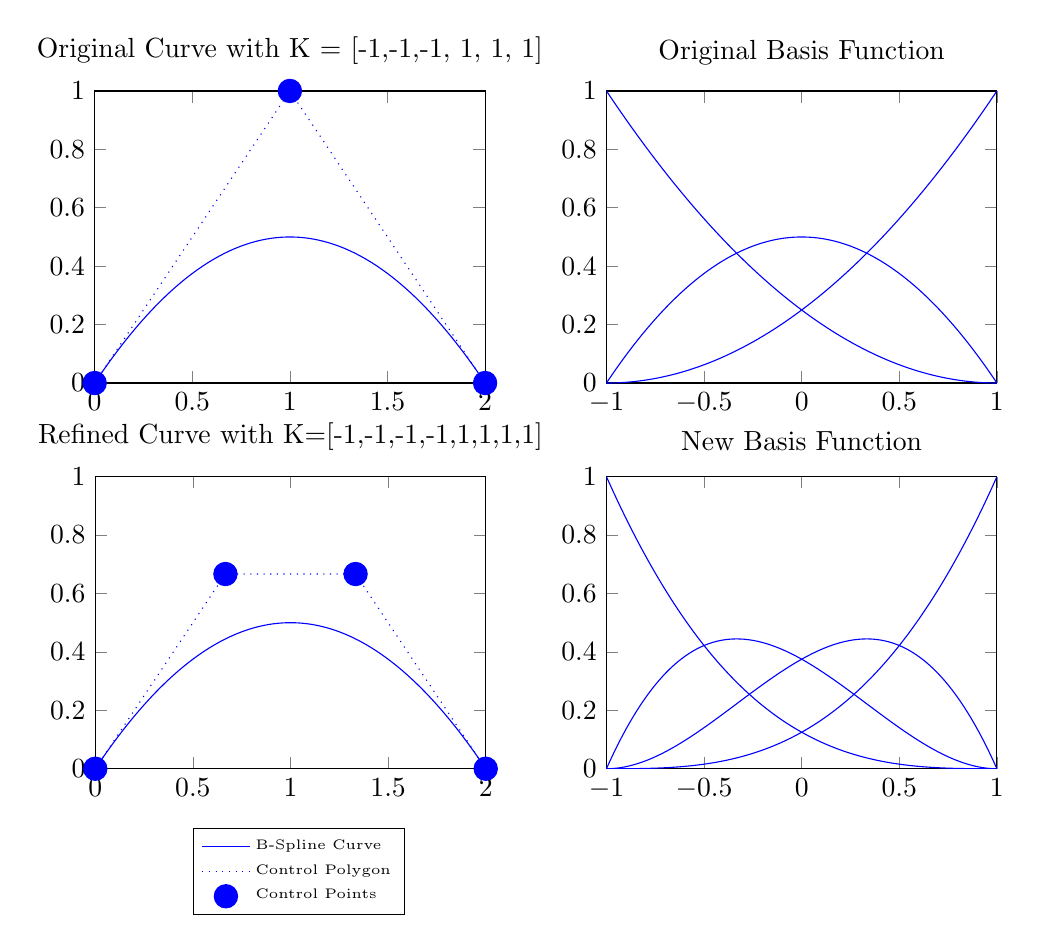
\begin{tikzpicture}[scale=1]

\begin{axis}[%
width=1.95217803030303in,
height=1.46030765503876in,
scale only axis,
xmin=0,
xmax=2,
ymin=0,
ymax=1,
name=plot1,
title={Original  Curve  with  K = [-1,-1,-1, 1, 1, 1]}
]
\addplot [color=blue,solid,forget plot]
  table[row sep=crcr]{
0	0	\\
0.0100502512562815	0.00999974748112426	\\
0.0201005025125628	0.019898487411934	\\
0.0301507537688442	0.0296962197924295	\\
0.0402010050251256	0.0393929446226105	\\
0.050251256281407	0.0489886619024772	\\
0.0603015075376885	0.0584833716320295	\\
0.0703517587939698	0.0678770738112674	\\
0.0804020100502513	0.0771697684401909	\\
0.0904522613065326	0.0863614555188	\\
0.100502512562814	0.0954521350470948	\\
0.110552763819096	0.104441807025075	\\
0.120603015075377	0.113330471452741	\\
0.130653266331658	0.122118128330093	\\
0.14070351758794	0.13080477765713	\\
0.150753768844221	0.139390419433853	\\
0.160804020100503	0.147875053660261	\\
0.170854271356784	0.156258680336355	\\
0.180904522613065	0.164541299462135	\\
0.190954773869347	0.1727229110376	\\
0.201005025125628	0.180803515062751	\\
0.21105527638191	0.188783111537587	\\
0.221105527638191	0.19666170046211	\\
0.231155778894472	0.204439281836317	\\
0.241206030150754	0.212115855660211	\\
0.251256281407035	0.21969142193379	\\
0.261306532663317	0.227165980657054	\\
0.271356783919598	0.234539531830004	\\
0.281407035175879	0.24181207545264	\\
0.291457286432161	0.248983611524961	\\
0.301507537688442	0.256054140046968	\\
0.311557788944724	0.263023661018661	\\
0.321608040201005	0.269892174440039	\\
0.331658291457286	0.276659680311103	\\
0.341708542713568	0.283326178631853	\\
0.351758793969849	0.289891669402288	\\
0.361809045226131	0.296356152622409	\\
0.371859296482412	0.302719628292215	\\
0.381909547738693	0.308982096411707	\\
0.391959798994975	0.315143556980884	\\
0.402010050251256	0.321204009999747	\\
0.412060301507538	0.327163455468296	\\
0.422110552763819	0.333021893386531	\\
0.4321608040201	0.338779323754451	\\
0.442211055276382	0.344435746572056	\\
0.452261306532663	0.349991161839347	\\
0.462311557788945	0.355445569556324	\\
0.472361809045226	0.360798969722987	\\
0.482412060301508	0.366051362339335	\\
0.492462311557789	0.371202747405369	\\
0.50251256281407	0.376253124921088	\\
0.512562814070352	0.381202494886493	\\
0.522613065326633	0.386050857301583	\\
0.532663316582915	0.390798212166359	\\
0.542713567839196	0.395444559480821	\\
0.552763819095477	0.399989899244969	\\
0.562814070351759	0.404434231458802	\\
0.57286432160804	0.40877755612232	\\
0.582914572864322	0.413019873235524	\\
0.592964824120603	0.417161182798414	\\
0.603015075376884	0.42120148481099	\\
0.613065326633166	0.425140779273251	\\
0.623115577889447	0.428979066185197	\\
0.633165829145729	0.43271634554683	\\
0.64321608040201	0.436352617358148	\\
0.653266331658292	0.439887881619151	\\
0.663316582914573	0.44332213832984	\\
0.673366834170854	0.446655387490215	\\
0.683417085427136	0.449887629100275	\\
0.693467336683417	0.453018863160021	\\
0.703517587939699	0.456049089669453	\\
0.71356783919598	0.45897830862857	\\
0.723618090452261	0.461806520037373	\\
0.733668341708543	0.464533723895861	\\
0.743718592964824	0.467159920204035	\\
0.753768844221106	0.469685108961895	\\
0.763819095477387	0.47210929016944	\\
0.773869346733668	0.474432463826671	\\
0.78391959798995	0.476654629933588	\\
0.793969849246231	0.47877578849019	\\
0.804020100502513	0.480795939496477	\\
0.814070351758794	0.482715082952451	\\
0.824120603015075	0.48453321885811	\\
0.834170854271357	0.486250347213454	\\
0.844221105527638	0.487866468018484	\\
0.85427135678392	0.4893815812732	\\
0.864321608040201	0.490795686977602	\\
0.874371859296482	0.492108785131689	\\
0.884422110552764	0.493320875735461	\\
0.894472361809045	0.494431958788919	\\
0.904522613065327	0.495442034292063	\\
0.914572864321608	0.496351102244893	\\
0.924623115577889	0.497159162647408	\\
0.934673366834171	0.497866215499609	\\
0.944723618090452	0.498472260801495	\\
0.954773869346734	0.498977298553067	\\
0.964824120603015	0.499381328754324	\\
0.974874371859296	0.499684351405268	\\
0.984924623115578	0.499886366505896	\\
0.994974874371859	0.499987374056211	\\
1.00502512562814	0.499987374056211	\\
1.01507537688442	0.499886366505896	\\
1.0251256281407	0.499684351405268	\\
1.03517587939699	0.499381328754324	\\
1.04522613065327	0.498977298553067	\\
1.05527638190955	0.498472260801495	\\
1.06532663316583	0.497866215499609	\\
1.07537688442211	0.497159162647408	\\
1.08542713567839	0.496351102244893	\\
1.09547738693467	0.495442034292063	\\
1.10552763819095	0.494431958788919	\\
1.11557788944724	0.493320875735461	\\
1.12562814070352	0.492108785131689	\\
1.1356783919598	0.490795686977602	\\
1.14572864321608	0.4893815812732	\\
1.15577889447236	0.487866468018484	\\
1.16582914572864	0.486250347213454	\\
1.17587939698492	0.48453321885811	\\
1.18592964824121	0.482715082952451	\\
1.19597989949749	0.480795939496477	\\
1.20603015075377	0.47877578849019	\\
1.21608040201005	0.476654629933588	\\
1.22613065326633	0.474432463826671	\\
1.23618090452261	0.47210929016944	\\
1.24623115577889	0.469685108961895	\\
1.25628140703518	0.467159920204035	\\
1.26633165829146	0.464533723895861	\\
1.27638190954774	0.461806520037373	\\
1.28643216080402	0.45897830862857	\\
1.2964824120603	0.456049089669453	\\
1.30653266331658	0.453018863160021	\\
1.31658291457286	0.449887629100275	\\
1.32663316582915	0.446655387490215	\\
1.33668341708543	0.44332213832984	\\
1.34673366834171	0.439887881619151	\\
1.35678391959799	0.436352617358148	\\
1.36683417085427	0.43271634554683	\\
1.37688442211055	0.428979066185197	\\
1.38693467336683	0.425140779273251	\\
1.39698492462312	0.42120148481099	\\
1.4070351758794	0.417161182798414	\\
1.41708542713568	0.413019873235524	\\
1.42713567839196	0.40877755612232	\\
1.43718592964824	0.404434231458802	\\
1.44723618090452	0.399989899244969	\\
1.4572864321608	0.395444559480821	\\
1.46733668341709	0.390798212166359	\\
1.47738693467337	0.386050857301583	\\
1.48743718592965	0.381202494886493	\\
1.49748743718593	0.376253124921088	\\
1.50753768844221	0.371202747405369	\\
1.51758793969849	0.366051362339335	\\
1.52763819095477	0.360798969722987	\\
1.53768844221106	0.355445569556324	\\
1.54773869346734	0.349991161839347	\\
1.55778894472362	0.344435746572056	\\
1.5678391959799	0.338779323754451	\\
1.57788944723618	0.333021893386531	\\
1.58793969849246	0.327163455468296	\\
1.59798994974874	0.321204009999747	\\
1.60804020100503	0.315143556980884	\\
1.61809045226131	0.308982096411707	\\
1.62814070351759	0.302719628292215	\\
1.63819095477387	0.296356152622409	\\
1.64824120603015	0.289891669402288	\\
1.65829145728643	0.283326178631853	\\
1.66834170854271	0.276659680311103	\\
1.67839195979899	0.269892174440039	\\
1.68844221105528	0.263023661018661	\\
1.69849246231156	0.256054140046968	\\
1.70854271356784	0.248983611524961	\\
1.71859296482412	0.24181207545264	\\
1.7286432160804	0.234539531830004	\\
1.73869346733668	0.227165980657054	\\
1.74874371859296	0.21969142193379	\\
1.75879396984925	0.212115855660211	\\
1.76884422110553	0.204439281836317	\\
1.77889447236181	0.19666170046211	\\
1.78894472361809	0.188783111537587	\\
1.79899497487437	0.180803515062751	\\
1.80904522613065	0.1727229110376	\\
1.81909547738693	0.164541299462135	\\
1.82914572864322	0.156258680336355	\\
1.8391959798995	0.147875053660261	\\
1.84924623115578	0.139390419433853	\\
1.85929648241206	0.13080477765713	\\
1.86934673366834	0.122118128330093	\\
1.87939698492462	0.113330471452741	\\
1.8894472361809	0.104441807025075	\\
1.89949748743719	0.0954521350470948	\\
1.90954773869347	0.0863614555188	\\
1.91959798994975	0.0771697684401908	\\
1.92964824120603	0.0678770738112675	\\
1.93969849246231	0.0584833716320295	\\
1.94974874371859	0.0489886619024772	\\
1.95979899497487	0.0393929446226105	\\
1.96984924623116	0.0296962197924294	\\
1.97989949748744	0.0198984874119341	\\
1.98994974874372	0.00999974748112426	\\
2	0	\\
};
\addplot [color=blue,dotted,forget plot]
  table[row sep=crcr]{
0	0	\\
1	1	\\
2	0	\\
};
\addplot [color=blue,mark size=4.2pt,only marks,mark=*,mark options={solid},forget plot]
  table[row sep=crcr]{
0	0	\\
1	1	\\
2	0	\\
};
\end{axis}

\begin{axis}[%
width=1.95217803030303in,
height=1.46030765503876in,
scale only axis,
xmin=-1,
xmax=1,
ymin=0,
ymax=1,
name=plot2,
at=(plot1.right of south east),
anchor=left of south west,
title={Original Basis Function}
]
\addplot [color=blue,solid,forget plot]
  table[row sep=crcr]{
-1	1	\\
-0.989949748743719	0.989975000631297	\\
-0.979899497487437	0.980000505037751	\\
-0.969849246231156	0.970076513219363	\\
-0.959798994974874	0.960203025176132	\\
-0.949748743718593	0.950380040908058	\\
-0.939698492462312	0.940607560415141	\\
-0.92964824120603	0.930885583697381	\\
-0.919597989949749	0.921214110754779	\\
-0.909547738693467	0.911593141587334	\\
-0.899497487437186	0.902022676195046	\\
-0.889447236180904	0.892502714577915	\\
-0.879396984924623	0.883033256735941	\\
-0.869346733668342	0.873614302669125	\\
-0.85929648241206	0.864245852377465	\\
-0.849246231155779	0.854927905860963	\\
-0.839195979899497	0.845660463119618	\\
-0.829145728643216	0.83644352415343	\\
-0.819095477386935	0.8272770889624	\\
-0.809045226130653	0.818161157546527	\\
-0.798994974874372	0.80909572990581	\\
-0.78894472361809	0.800080806040251	\\
-0.778894472361809	0.79111638594985	\\
-0.768844221105528	0.782202469634605	\\
-0.758793969849246	0.773339057094518	\\
-0.748743718592965	0.764526148329588	\\
-0.738693467336683	0.755763743339815	\\
-0.728643216080402	0.747051842125199	\\
-0.718592964824121	0.73839044468574	\\
-0.708542713567839	0.729779551021439	\\
-0.698492462311558	0.721219161132295	\\
-0.688442211055276	0.712709275018308	\\
-0.678391959798995	0.704249892679478	\\
-0.668341708542714	0.695841014115805	\\
-0.658291457286432	0.68748263932729	\\
-0.648241206030151	0.679174768313932	\\
-0.638190954773869	0.67091740107573	\\
-0.628140703517588	0.662710537612687	\\
-0.618090452261307	0.6545541779248	\\
-0.608040201005025	0.64644832201207	\\
-0.597989949748744	0.638392969874498	\\
-0.587939698492462	0.630388121512083	\\
-0.577889447236181	0.622433776924825	\\
-0.5678391959799	0.614529936112725	\\
-0.557788944723618	0.606676599075781	\\
-0.547738693467337	0.598873765813995	\\
-0.537688442211055	0.591121436327365	\\
-0.527638190954774	0.583419610615894	\\
-0.517587939698492	0.575768288679579	\\
-0.507537688442211	0.568167470518421	\\
-0.49748743718593	0.560617156132421	\\
-0.487437185929648	0.553117345521578	\\
-0.477386934673367	0.545668038685892	\\
-0.467336683417085	0.538269235625363	\\
-0.457286432160804	0.530920936339991	\\
-0.447236180904523	0.523623140829777	\\
-0.437185929648241	0.51637584909472	\\
-0.42713567839196	0.50917906113482	\\
-0.417085427135678	0.502032776950077	\\
-0.407035175879397	0.494936996540491	\\
-0.396984924623116	0.487891719906063	\\
-0.386934673366834	0.480896947046792	\\
-0.376884422110553	0.473952677962678	\\
-0.366834170854271	0.467058912653721	\\
-0.35678391959799	0.460215651119921	\\
-0.346733668341708	0.453422893361279	\\
-0.336683417085427	0.446680639377794	\\
-0.326633165829146	0.439988889169465	\\
-0.316582914572864	0.433347642736295	\\
-0.306532663316583	0.426756900078281	\\
-0.296482412060301	0.420216661195424	\\
-0.28643216080402	0.413726926087725	\\
-0.276381909547739	0.407287694755183	\\
-0.266331658291457	0.400898967197798	\\
-0.256281407035176	0.39456074341557	\\
-0.246231155778894	0.3882730234085	\\
-0.236180904522613	0.382035807176586	\\
-0.226130653266332	0.37584909471983	\\
-0.21608040201005	0.369712886038231	\\
-0.206030150753769	0.36362718113179	\\
-0.195979899497487	0.357591980000505	\\
-0.185929648241206	0.351607282644378	\\
-0.175879396984925	0.345673089063407	\\
-0.165829145728643	0.339789399257595	\\
-0.155778894472362	0.333956213226939	\\
-0.14572864321608	0.32817353097144	\\
-0.135678391959799	0.322441352491099	\\
-0.125628140703518	0.316759677785915	\\
-0.115577889447236	0.311128506855887	\\
-0.105527638190955	0.305547839701018	\\
-0.0954773869346733	0.300017676321305	\\
-0.085427135678392	0.29453801671675	\\
-0.0753768844221105	0.289108860887351	\\
-0.0653266331658291	0.28373020883311	\\
-0.0552763819095478	0.278402060554026	\\
-0.0452261306532663	0.2731244160501	\\
-0.035175879396985	0.26789727532133	\\
-0.0251256281407035	0.262720638367718	\\
-0.0150753768844221	0.257594505189263	\\
-0.00502512562814073	0.252518875785965	\\
0.00502512562814061	0.247493750157824	\\
0.0150753768844221	0.242519128304841	\\
0.0251256281407035	0.237595010227014	\\
0.035175879396985	0.232721395924345	\\
0.0452261306532664	0.227898285396833	\\
0.0552763819095476	0.223125678644479	\\
0.0653266331658291	0.218403575667281	\\
0.0753768844221105	0.213731976465241	\\
0.085427135678392	0.209110881038358	\\
0.0954773869346734	0.204540289386632	\\
0.105527638190955	0.200020201510063	\\
0.115577889447236	0.195550617408651	\\
0.125628140703518	0.191131537082397	\\
0.135678391959799	0.1867629605313	\\
0.14572864321608	0.18244488775536	\\
0.155778894472362	0.178177318754577	\\
0.165829145728643	0.173960253528951	\\
0.175879396984925	0.169793692078483	\\
0.185929648241206	0.165677634403172	\\
0.195979899497488	0.161612080503018	\\
0.206030150753769	0.157597030378021	\\
0.21608040201005	0.153632484028181	\\
0.226130653266332	0.149718441453499	\\
0.236180904522613	0.145854902653973	\\
0.246231155778895	0.142041867629605	\\
0.256281407035176	0.138279336380394	\\
0.266331658291457	0.134567308906341	\\
0.276381909547739	0.130905785207444	\\
0.28643216080402	0.127294765283705	\\
0.296482412060302	0.123734249135123	\\
0.306532663316583	0.120224236761698	\\
0.316582914572864	0.11676472816343	\\
0.326633165829146	0.11335572334032	\\
0.336683417085427	0.109997222292366	\\
0.346733668341709	0.10668922501957	\\
0.35678391959799	0.103431731521931	\\
0.366834170854271	0.10022474179945	\\
0.376884422110553	0.097068255852125	\\
0.386934673366834	0.0939622736799576	\\
0.396984924623116	0.0909067952829474	\\
0.407035175879397	0.0879018206610944	\\
0.417085427135678	0.0849473498143987	\\
0.42713567839196	0.08204338274286	\\
0.437185929648241	0.0791899194464786	\\
0.447236180904523	0.0763869599252544	\\
0.457286432160804	0.0736345041791874	\\
0.467336683417085	0.0709325522082776	\\
0.477386934673367	0.0682811040125249	\\
0.487437185929648	0.0656801595919295	\\
0.49748743718593	0.0631297189464912	\\
0.507537688442211	0.0606297820762102	\\
0.517587939698492	0.0581803489810864	\\
0.527638190954774	0.0557814196611197	\\
0.537688442211055	0.0534329941163102	\\
0.547738693467337	0.0511350723466579	\\
0.557788944723618	0.0488876543521628	\\
0.567839195979899	0.0466907401328249	\\
0.577889447236181	0.0445443296886442	\\
0.587939698492462	0.0424484230196207	\\
0.597989949748744	0.0404030201257544	\\
0.608040201005025	0.0384081210070453	\\
0.618090452261306	0.0364637256634934	\\
0.628140703517588	0.0345698340950986	\\
0.638190954773869	0.0327264463018611	\\
0.648241206030151	0.0309335622837807	\\
0.658291457286432	0.0291911820408575	\\
0.668341708542713	0.0274993055730916	\\
0.678391959798995	0.0258579328804828	\\
0.688442211055276	0.0242670639630312	\\
0.698492462311558	0.0227266988207368	\\
0.708542713567839	0.0212368374535996	\\
0.71859296482412	0.0197974798616197	\\
0.728643216080402	0.0184086260447969	\\
0.738693467336683	0.0170702760031312	\\
0.748743718592965	0.0157824297366228	\\
0.758793969849246	0.0145450872452716	\\
0.768844221105528	0.0133582485290775	\\
0.778894472361809	0.0122219135880407	\\
0.78894472361809	0.0111360824221611	\\
0.798994974874372	0.0101007550314386	\\
0.809045226130653	0.00911593141587333	\\
0.819095477386935	0.00818161157546526	\\
0.829145728643216	0.0072977955102144	\\
0.839195979899497	0.00646448322012071	\\
0.849246231155779	0.00568167470518421	\\
0.85929648241206	0.00494936996540491	\\
0.869346733668342	0.0042675690007828	\\
0.879396984924623	0.0036362718113179	\\
0.889447236180904	0.00305547839701018	\\
0.899497487437186	0.00252518875785965	\\
0.909547738693467	0.00204540289386631	\\
0.919597989949749	0.00161612080503017	\\
0.92964824120603	0.00123734249135123	\\
0.939698492462312	0.000909067952829475	\\
0.949748743718593	0.000631297189464912	\\
0.959798994974874	0.000404030201257543	\\
0.969849246231156	0.000227266988207367	\\
0.979899497487437	0.000101007550314387	\\
0.989949748743719	2.52518875785967e-05	\\
1	0	\\
};
\addplot [color=blue,solid,forget plot]
  table[row sep=crcr]{
-1	0	\\
-0.989949748743719	0.00999974748112426	\\
-0.979899497487437	0.019898487411934	\\
-0.969849246231156	0.0296962197924295	\\
-0.959798994974874	0.0393929446226105	\\
-0.949748743718593	0.0489886619024772	\\
-0.939698492462312	0.0584833716320295	\\
-0.92964824120603	0.0678770738112674	\\
-0.919597989949749	0.0771697684401909	\\
-0.909547738693467	0.0863614555188	\\
-0.899497487437186	0.0954521350470948	\\
-0.889447236180904	0.104441807025075	\\
-0.879396984924623	0.113330471452741	\\
-0.869346733668342	0.122118128330093	\\
-0.85929648241206	0.13080477765713	\\
-0.849246231155779	0.139390419433853	\\
-0.839195979899497	0.147875053660261	\\
-0.829145728643216	0.156258680336355	\\
-0.819095477386935	0.164541299462135	\\
-0.809045226130653	0.1727229110376	\\
-0.798994974874372	0.180803515062751	\\
-0.78894472361809	0.188783111537587	\\
-0.778894472361809	0.19666170046211	\\
-0.768844221105528	0.204439281836317	\\
-0.758793969849246	0.212115855660211	\\
-0.748743718592965	0.21969142193379	\\
-0.738693467336683	0.227165980657054	\\
-0.728643216080402	0.234539531830004	\\
-0.718592964824121	0.24181207545264	\\
-0.708542713567839	0.248983611524961	\\
-0.698492462311558	0.256054140046968	\\
-0.688442211055276	0.263023661018661	\\
-0.678391959798995	0.269892174440039	\\
-0.668341708542714	0.276659680311103	\\
-0.658291457286432	0.283326178631853	\\
-0.648241206030151	0.289891669402288	\\
-0.638190954773869	0.296356152622409	\\
-0.628140703517588	0.302719628292215	\\
-0.618090452261307	0.308982096411707	\\
-0.608040201005025	0.315143556980884	\\
-0.597989949748744	0.321204009999747	\\
-0.587939698492462	0.327163455468296	\\
-0.577889447236181	0.333021893386531	\\
-0.5678391959799	0.338779323754451	\\
-0.557788944723618	0.344435746572056	\\
-0.547738693467337	0.349991161839347	\\
-0.537688442211055	0.355445569556324	\\
-0.527638190954774	0.360798969722987	\\
-0.517587939698492	0.366051362339335	\\
-0.507537688442211	0.371202747405369	\\
-0.49748743718593	0.376253124921088	\\
-0.487437185929648	0.381202494886493	\\
-0.477386934673367	0.386050857301583	\\
-0.467336683417085	0.390798212166359	\\
-0.457286432160804	0.395444559480821	\\
-0.447236180904523	0.399989899244969	\\
-0.437185929648241	0.404434231458802	\\
-0.42713567839196	0.40877755612232	\\
-0.417085427135678	0.413019873235524	\\
-0.407035175879397	0.417161182798414	\\
-0.396984924623116	0.42120148481099	\\
-0.386934673366834	0.425140779273251	\\
-0.376884422110553	0.428979066185197	\\
-0.366834170854271	0.43271634554683	\\
-0.35678391959799	0.436352617358148	\\
-0.346733668341708	0.439887881619151	\\
-0.336683417085427	0.44332213832984	\\
-0.326633165829146	0.446655387490215	\\
-0.316582914572864	0.449887629100275	\\
-0.306532663316583	0.453018863160021	\\
-0.296482412060301	0.456049089669453	\\
-0.28643216080402	0.45897830862857	\\
-0.276381909547739	0.461806520037373	\\
-0.266331658291457	0.464533723895861	\\
-0.256281407035176	0.467159920204035	\\
-0.246231155778894	0.469685108961895	\\
-0.236180904522613	0.47210929016944	\\
-0.226130653266332	0.474432463826671	\\
-0.21608040201005	0.476654629933588	\\
-0.206030150753769	0.47877578849019	\\
-0.195979899497487	0.480795939496477	\\
-0.185929648241206	0.482715082952451	\\
-0.175879396984925	0.48453321885811	\\
-0.165829145728643	0.486250347213454	\\
-0.155778894472362	0.487866468018484	\\
-0.14572864321608	0.4893815812732	\\
-0.135678391959799	0.490795686977602	\\
-0.125628140703518	0.492108785131689	\\
-0.115577889447236	0.493320875735461	\\
-0.105527638190955	0.494431958788919	\\
-0.0954773869346733	0.495442034292063	\\
-0.085427135678392	0.496351102244893	\\
-0.0753768844221105	0.497159162647408	\\
-0.0653266331658291	0.497866215499609	\\
-0.0552763819095478	0.498472260801495	\\
-0.0452261306532663	0.498977298553067	\\
-0.035175879396985	0.499381328754324	\\
-0.0251256281407035	0.499684351405268	\\
-0.0150753768844221	0.499886366505896	\\
-0.00502512562814073	0.499987374056211	\\
0.00502512562814061	0.499987374056211	\\
0.0150753768844221	0.499886366505896	\\
0.0251256281407035	0.499684351405268	\\
0.035175879396985	0.499381328754324	\\
0.0452261306532664	0.498977298553067	\\
0.0552763819095476	0.498472260801495	\\
0.0653266331658291	0.497866215499609	\\
0.0753768844221105	0.497159162647408	\\
0.085427135678392	0.496351102244893	\\
0.0954773869346734	0.495442034292063	\\
0.105527638190955	0.494431958788919	\\
0.115577889447236	0.493320875735461	\\
0.125628140703518	0.492108785131689	\\
0.135678391959799	0.490795686977602	\\
0.14572864321608	0.4893815812732	\\
0.155778894472362	0.487866468018484	\\
0.165829145728643	0.486250347213454	\\
0.175879396984925	0.48453321885811	\\
0.185929648241206	0.482715082952451	\\
0.195979899497488	0.480795939496477	\\
0.206030150753769	0.47877578849019	\\
0.21608040201005	0.476654629933588	\\
0.226130653266332	0.474432463826671	\\
0.236180904522613	0.47210929016944	\\
0.246231155778895	0.469685108961895	\\
0.256281407035176	0.467159920204035	\\
0.266331658291457	0.464533723895861	\\
0.276381909547739	0.461806520037373	\\
0.28643216080402	0.45897830862857	\\
0.296482412060302	0.456049089669453	\\
0.306532663316583	0.453018863160021	\\
0.316582914572864	0.449887629100275	\\
0.326633165829146	0.446655387490215	\\
0.336683417085427	0.44332213832984	\\
0.346733668341709	0.439887881619151	\\
0.35678391959799	0.436352617358148	\\
0.366834170854271	0.43271634554683	\\
0.376884422110553	0.428979066185197	\\
0.386934673366834	0.425140779273251	\\
0.396984924623116	0.42120148481099	\\
0.407035175879397	0.417161182798414	\\
0.417085427135678	0.413019873235524	\\
0.42713567839196	0.40877755612232	\\
0.437185929648241	0.404434231458802	\\
0.447236180904523	0.399989899244969	\\
0.457286432160804	0.395444559480821	\\
0.467336683417085	0.390798212166359	\\
0.477386934673367	0.386050857301583	\\
0.487437185929648	0.381202494886493	\\
0.49748743718593	0.376253124921088	\\
0.507537688442211	0.371202747405369	\\
0.517587939698492	0.366051362339335	\\
0.527638190954774	0.360798969722987	\\
0.537688442211055	0.355445569556324	\\
0.547738693467337	0.349991161839347	\\
0.557788944723618	0.344435746572056	\\
0.567839195979899	0.338779323754451	\\
0.577889447236181	0.333021893386531	\\
0.587939698492462	0.327163455468296	\\
0.597989949748744	0.321204009999747	\\
0.608040201005025	0.315143556980884	\\
0.618090452261306	0.308982096411707	\\
0.628140703517588	0.302719628292215	\\
0.638190954773869	0.296356152622409	\\
0.648241206030151	0.289891669402288	\\
0.658291457286432	0.283326178631853	\\
0.668341708542713	0.276659680311103	\\
0.678391959798995	0.269892174440039	\\
0.688442211055276	0.263023661018661	\\
0.698492462311558	0.256054140046968	\\
0.708542713567839	0.248983611524961	\\
0.71859296482412	0.24181207545264	\\
0.728643216080402	0.234539531830004	\\
0.738693467336683	0.227165980657054	\\
0.748743718592965	0.21969142193379	\\
0.758793969849246	0.212115855660211	\\
0.768844221105528	0.204439281836317	\\
0.778894472361809	0.19666170046211	\\
0.78894472361809	0.188783111537587	\\
0.798994974874372	0.180803515062751	\\
0.809045226130653	0.1727229110376	\\
0.819095477386935	0.164541299462135	\\
0.829145728643216	0.156258680336355	\\
0.839195979899497	0.147875053660261	\\
0.849246231155779	0.139390419433853	\\
0.85929648241206	0.13080477765713	\\
0.869346733668342	0.122118128330093	\\
0.879396984924623	0.113330471452741	\\
0.889447236180904	0.104441807025075	\\
0.899497487437186	0.0954521350470948	\\
0.909547738693467	0.0863614555188	\\
0.919597989949749	0.0771697684401908	\\
0.92964824120603	0.0678770738112675	\\
0.939698492462312	0.0584833716320295	\\
0.949748743718593	0.0489886619024772	\\
0.959798994974874	0.0393929446226105	\\
0.969849246231156	0.0296962197924294	\\
0.979899497487437	0.0198984874119341	\\
0.989949748743719	0.00999974748112426	\\
1	0	\\
};
\addplot [color=blue,solid,forget plot]
  table[row sep=crcr]{
-1	0	\\
-0.989949748743719	2.52518875785967e-05	\\
-0.979899497487437	0.000101007550314386	\\
-0.969849246231156	0.000227266988207369	\\
-0.959798994974874	0.000404030201257543	\\
-0.949748743718593	0.000631297189464912	\\
-0.939698492462312	0.000909067952829475	\\
-0.92964824120603	0.00123734249135123	\\
-0.919597989949749	0.00161612080503018	\\
-0.909547738693467	0.00204540289386631	\\
-0.899497487437186	0.00252518875785965	\\
-0.889447236180904	0.00305547839701018	\\
-0.879396984924623	0.00363627181131789	\\
-0.869346733668342	0.00426756900078281	\\
-0.85929648241206	0.00494936996540491	\\
-0.849246231155779	0.00568167470518421	\\
-0.839195979899497	0.00646448322012071	\\
-0.829145728643216	0.00729779551021439	\\
-0.819095477386935	0.00818161157546527	\\
-0.809045226130653	0.00911593141587333	\\
-0.798994974874372	0.0101007550314386	\\
-0.78894472361809	0.0111360824221611	\\
-0.778894472361809	0.0122219135880407	\\
-0.768844221105528	0.0133582485290775	\\
-0.758793969849246	0.0145450872452716	\\
-0.748743718592965	0.0157824297366228	\\
-0.738693467336683	0.0170702760031312	\\
-0.728643216080402	0.0184086260447969	\\
-0.718592964824121	0.0197974798616197	\\
-0.708542713567839	0.0212368374535996	\\
-0.698492462311558	0.0227266988207368	\\
-0.688442211055276	0.0242670639630312	\\
-0.678391959798995	0.0258579328804828	\\
-0.668341708542714	0.0274993055730916	\\
-0.658291457286432	0.0291911820408575	\\
-0.648241206030151	0.0309335622837807	\\
-0.638190954773869	0.0327264463018611	\\
-0.628140703517588	0.0345698340950986	\\
-0.618090452261307	0.0364637256634933	\\
-0.608040201005025	0.0384081210070453	\\
-0.597989949748744	0.0404030201257544	\\
-0.587939698492462	0.0424484230196207	\\
-0.577889447236181	0.0445443296886442	\\
-0.5678391959799	0.0466907401328249	\\
-0.557788944723618	0.0488876543521628	\\
-0.547738693467337	0.0511350723466579	\\
-0.537688442211055	0.0534329941163102	\\
-0.527638190954774	0.0557814196611197	\\
-0.517587939698492	0.0581803489810863	\\
-0.507537688442211	0.0606297820762102	\\
-0.49748743718593	0.0631297189464912	\\
-0.487437185929648	0.0656801595919295	\\
-0.477386934673367	0.0682811040125249	\\
-0.467336683417085	0.0709325522082776	\\
-0.457286432160804	0.0736345041791874	\\
-0.447236180904523	0.0763869599252544	\\
-0.437185929648241	0.0791899194464786	\\
-0.42713567839196	0.08204338274286	\\
-0.417085427135678	0.0849473498143986	\\
-0.407035175879397	0.0879018206610944	\\
-0.396984924623116	0.0909067952829474	\\
-0.386934673366834	0.0939622736799576	\\
-0.376884422110553	0.097068255852125	\\
-0.366834170854271	0.10022474179945	\\
-0.35678391959799	0.103431731521931	\\
-0.346733668341708	0.10668922501957	\\
-0.336683417085427	0.109997222292366	\\
-0.326633165829146	0.11335572334032	\\
-0.316582914572864	0.11676472816343	\\
-0.306532663316583	0.120224236761698	\\
-0.296482412060301	0.123734249135123	\\
-0.28643216080402	0.127294765283705	\\
-0.276381909547739	0.130905785207444	\\
-0.266331658291457	0.134567308906341	\\
-0.256281407035176	0.138279336380394	\\
-0.246231155778894	0.142041867629605	\\
-0.236180904522613	0.145854902653973	\\
-0.226130653266332	0.149718441453499	\\
-0.21608040201005	0.153632484028181	\\
-0.206030150753769	0.157597030378021	\\
-0.195979899497487	0.161612080503018	\\
-0.185929648241206	0.165677634403172	\\
-0.175879396984925	0.169793692078483	\\
-0.165829145728643	0.173960253528951	\\
-0.155778894472362	0.178177318754577	\\
-0.14572864321608	0.18244488775536	\\
-0.135678391959799	0.1867629605313	\\
-0.125628140703518	0.191131537082397	\\
-0.115577889447236	0.195550617408651	\\
-0.105527638190955	0.200020201510063	\\
-0.0954773869346733	0.204540289386632	\\
-0.085427135678392	0.209110881038358	\\
-0.0753768844221105	0.213731976465241	\\
-0.0653266331658291	0.218403575667281	\\
-0.0552763819095478	0.223125678644479	\\
-0.0452261306532663	0.227898285396833	\\
-0.035175879396985	0.232721395924345	\\
-0.0251256281407035	0.237595010227014	\\
-0.0150753768844221	0.242519128304841	\\
-0.00502512562814073	0.247493750157824	\\
0.00502512562814061	0.252518875785965	\\
0.0150753768844221	0.257594505189263	\\
0.0251256281407035	0.262720638367718	\\
0.035175879396985	0.26789727532133	\\
0.0452261306532664	0.2731244160501	\\
0.0552763819095476	0.278402060554026	\\
0.0653266331658291	0.28373020883311	\\
0.0753768844221105	0.289108860887351	\\
0.085427135678392	0.29453801671675	\\
0.0954773869346734	0.300017676321305	\\
0.105527638190955	0.305547839701018	\\
0.115577889447236	0.311128506855887	\\
0.125628140703518	0.316759677785915	\\
0.135678391959799	0.322441352491099	\\
0.14572864321608	0.32817353097144	\\
0.155778894472362	0.333956213226939	\\
0.165829145728643	0.339789399257594	\\
0.175879396984925	0.345673089063407	\\
0.185929648241206	0.351607282644378	\\
0.195979899497488	0.357591980000505	\\
0.206030150753769	0.36362718113179	\\
0.21608040201005	0.369712886038231	\\
0.226130653266332	0.37584909471983	\\
0.236180904522613	0.382035807176586	\\
0.246231155778895	0.3882730234085	\\
0.256281407035176	0.39456074341557	\\
0.266331658291457	0.400898967197798	\\
0.276381909547739	0.407287694755183	\\
0.28643216080402	0.413726926087725	\\
0.296482412060302	0.420216661195424	\\
0.306532663316583	0.426756900078281	\\
0.316582914572864	0.433347642736295	\\
0.326633165829146	0.439988889169465	\\
0.336683417085427	0.446680639377794	\\
0.346733668341709	0.453422893361279	\\
0.35678391959799	0.460215651119921	\\
0.366834170854271	0.467058912653721	\\
0.376884422110553	0.473952677962678	\\
0.386934673366834	0.480896947046792	\\
0.396984924623116	0.487891719906063	\\
0.407035175879397	0.494936996540491	\\
0.417085427135678	0.502032776950077	\\
0.42713567839196	0.50917906113482	\\
0.437185929648241	0.51637584909472	\\
0.447236180904523	0.523623140829777	\\
0.457286432160804	0.530920936339991	\\
0.467336683417085	0.538269235625363	\\
0.477386934673367	0.545668038685892	\\
0.487437185929648	0.553117345521578	\\
0.49748743718593	0.560617156132421	\\
0.507537688442211	0.568167470518421	\\
0.517587939698492	0.575768288679579	\\
0.527638190954774	0.583419610615894	\\
0.537688442211055	0.591121436327365	\\
0.547738693467337	0.598873765813995	\\
0.557788944723618	0.606676599075781	\\
0.567839195979899	0.614529936112724	\\
0.577889447236181	0.622433776924825	\\
0.587939698492462	0.630388121512083	\\
0.597989949748744	0.638392969874498	\\
0.608040201005025	0.64644832201207	\\
0.618090452261306	0.6545541779248	\\
0.628140703517588	0.662710537612687	\\
0.638190954773869	0.67091740107573	\\
0.648241206030151	0.679174768313932	\\
0.658291457286432	0.68748263932729	\\
0.668341708542713	0.695841014115805	\\
0.678391959798995	0.704249892679478	\\
0.688442211055276	0.712709275018308	\\
0.698492462311558	0.721219161132295	\\
0.708542713567839	0.729779551021439	\\
0.71859296482412	0.73839044468574	\\
0.728643216080402	0.747051842125199	\\
0.738693467336683	0.755763743339815	\\
0.748743718592965	0.764526148329588	\\
0.758793969849246	0.773339057094518	\\
0.768844221105528	0.782202469634605	\\
0.778894472361809	0.79111638594985	\\
0.78894472361809	0.800080806040251	\\
0.798994974874372	0.80909572990581	\\
0.809045226130653	0.818161157546527	\\
0.819095477386935	0.8272770889624	\\
0.829145728643216	0.83644352415343	\\
0.839195979899497	0.845660463119618	\\
0.849246231155779	0.854927905860963	\\
0.85929648241206	0.864245852377465	\\
0.869346733668342	0.873614302669125	\\
0.879396984924623	0.883033256735941	\\
0.889447236180904	0.892502714577915	\\
0.899497487437186	0.902022676195046	\\
0.909547738693467	0.911593141587334	\\
0.919597989949749	0.921214110754779	\\
0.92964824120603	0.930885583697381	\\
0.939698492462312	0.940607560415141	\\
0.949748743718593	0.950380040908058	\\
0.959798994974874	0.960203025176132	\\
0.969849246231156	0.970076513219363	\\
0.979899497487437	0.980000505037751	\\
0.989949748743719	0.989975000631297	\\
1	1	\\
};
\end{axis}

\begin{axis}[%
width=1.95217803030303in,
height=1.46030765503876in,
scale only axis,
xmin=-1,
xmax=1,
ymin=0,
ymax=1,
name=plot4,
at=(plot2.below south west),
anchor=above north west,
title={New Basis Function}
]
\addplot [color=blue,solid,forget plot]
  table[row sep=crcr]{
-1	1	\\
-0.989949748743719	0.985000251884406	\\
-0.979899497487437	0.970151253730839	\\
-0.969849246231156	0.955452244175855	\\
-0.959798994974874	0.940902461856009	\\
-0.949748743718593	0.926501145407855	\\
-0.939698492462312	0.912247533467951	\\
-0.92964824120603	0.89814086467285	\\
-0.919597989949749	0.88418037765911	\\
-0.909547738693467	0.870365311063284	\\
-0.899497487437186	0.856694903521928	\\
-0.889447236180904	0.843168393671598	\\
-0.879396984924623	0.829785020148849	\\
-0.869346733668342	0.816544021590237	\\
-0.85929648241206	0.803444636632317	\\
-0.849246231155779	0.790486103911644	\\
-0.839195979899497	0.777667662064774	\\
-0.829145728643216	0.764988549728263	\\
-0.819095477386935	0.752448005538665	\\
-0.809045226130653	0.740045268132537	\\
-0.798994974874372	0.727779576146433	\\
-0.78894472361809	0.715650168216908	\\
-0.778894472361809	0.70365628298052	\\
-0.768844221105528	0.691797159073822	\\
-0.758793969849246	0.68007203513337	\\
-0.748743718592965	0.66848014979572	\\
-0.738693467336683	0.657020741697427	\\
-0.728643216080402	0.645693049475046	\\
-0.718592964824121	0.634496311765134	\\
-0.708542713567839	0.623429767204244	\\
-0.698492462311558	0.612492654428934	\\
-0.688442211055276	0.601684212075757	\\
-0.678391959798995	0.59100367878127	\\
-0.668341708542714	0.580450293182029	\\
-0.658291457286432	0.570023293914587	\\
-0.648241206030151	0.559721919615501	\\
-0.638190954773869	0.549545408921327	\\
-0.628140703517588	0.539493000468619	\\
-0.618090452261307	0.529563932893934	\\
-0.608040201005025	0.519757444833826	\\
-0.597989949748744	0.51007277492485	\\
-0.587939698492462	0.500509161803563	\\
-0.577889447236181	0.49106584410652	\\
-0.5678391959799	0.481742060470277	\\
-0.557788944723618	0.472537049531387	\\
-0.547738693467337	0.463450049926408	\\
-0.537688442211055	0.454480300291894	\\
-0.527638190954774	0.445627039264401	\\
-0.517587939698492	0.436889505480485	\\
-0.507537688442211	0.428266937576699	\\
-0.49748743718593	0.419758574189602	\\
-0.487437185929648	0.411363653955746	\\
-0.477386934673367	0.403081415511689	\\
-0.467336683417085	0.394911097493985	\\
-0.457286432160804	0.38685193853919	\\
-0.447236180904523	0.378903177283859	\\
-0.437185929648241	0.371064052364547	\\
-0.42713567839196	0.363333802417811	\\
-0.417085427135678	0.355711666080205	\\
-0.407035175879397	0.348196881988285	\\
-0.396984924623116	0.340788688778607	\\
-0.386934673366834	0.333486325087725	\\
-0.376884422110553	0.326289029552195	\\
-0.366834170854271	0.319196040808573	\\
-0.35678391959799	0.312206597493414	\\
-0.346733668341708	0.305319938243273	\\
-0.336683417085427	0.298535301694706	\\
-0.326633165829146	0.291851926484269	\\
-0.316582914572864	0.285269051248516	\\
-0.306532663316583	0.278785914624002	\\
-0.296482412060301	0.272401755247285	\\
-0.28643216080402	0.266115811754919	\\
-0.276381909547739	0.259927322783458	\\
-0.266331658291457	0.25383552696946	\\
-0.256281407035176	0.247839662949479	\\
-0.246231155778894	0.24193896936007	\\
-0.236180904522613	0.23613268483779	\\
-0.226130653266332	0.230420048019192	\\
-0.21608040201005	0.224800297540834	\\
-0.206030150753769	0.21927267203927	\\
-0.195979899497487	0.213836410151056	\\
-0.185929648241206	0.208490750512747	\\
-0.175879396984925	0.203234931760898	\\
-0.165829145728643	0.198068192532065	\\
-0.155778894472362	0.192989771462804	\\
-0.14572864321608	0.187998907189669	\\
-0.135678391959799	0.183094838349217	\\
-0.125628140703518	0.178276803578002	\\
-0.115577889447236	0.17354404151258	\\
-0.105527638190955	0.168895790789507	\\
-0.0954773869346733	0.164331290045338	\\
-0.085427135678392	0.159849777916628	\\
-0.0753768844221105	0.155450493039933	\\
-0.0653266331658291	0.151132674051807	\\
-0.0552763819095478	0.146895559588808	\\
-0.0452261306532663	0.142738388287489	\\
-0.035175879396985	0.138660398784407	\\
-0.0251256281407035	0.134660829716117	\\
-0.0150753768844221	0.130738919719174	\\
-0.00502512562814073	0.126893907430133	\\
0.00502512562814061	0.123125031485551	\\
0.0150753768844221	0.119431530521982	\\
0.0251256281407035	0.115812643175982	\\
0.035175879396985	0.112267608084106	\\
0.0452261306532664	0.10879566388291	\\
0.0552763819095476	0.10539604920895	\\
0.0653266331658291	0.10206800269878	\\
0.0753768844221105	0.0988107629889555	\\
0.085427135678392	0.0956235687160329	\\
0.0954773869346734	0.092505658516567	\\
0.105527638190955	0.0894562710271136	\\
0.115577889447236	0.0864746448842277	\\
0.125628140703518	0.083560018724465	\\
0.135678391959799	0.0807116311843808	\\
0.14572864321608	0.0779287209005305	\\
0.155778894472362	0.0752105265094697	\\
0.165829145728643	0.0725562866477536	\\
0.175879396984925	0.0699652399519377	\\
0.185929648241206	0.0674366250585774	\\
0.195979899497488	0.0649696806042282	\\
0.206030150753769	0.0625636452254455	\\
0.21608040201005	0.0602177575587846	\\
0.226130653266332	0.057931256240801	\\
0.236180904522613	0.0557033799080501	\\
0.246231155778895	0.0535333671970874	\\
0.256281407035176	0.0514204567444683	\\
0.266331658291457	0.0493638871867481	\\
0.276381909547739	0.0473628971604823	\\
0.28643216080402	0.0454167253022264	\\
0.296482412060302	0.0435246102485357	\\
0.306532663316583	0.0416857906359656	\\
0.316582914572864	0.0398995051010716	\\
0.326633165829146	0.0381649922804091	\\
0.336683417085427	0.0364814908105336	\\
0.346733668341709	0.0348482393280003	\\
0.35678391959799	0.0332644764693648	\\
0.366834170854271	0.0317294408711825	\\
0.376884422110553	0.0302423711700088	\\
0.386934673366834	0.0288025060023991	\\
0.396984924623116	0.0274090840049088	\\
0.407035175879397	0.0260613438140933	\\
0.417085427135678	0.0247585240665082	\\
0.42713567839196	0.0234998633987087	\\
0.437185929648241	0.0222846004472503	\\
0.447236180904523	0.0211119738486884	\\
0.457286432160804	0.0199812222395785	\\
0.467336683417085	0.0188915842564759	\\
0.477386934673367	0.0178422985359362	\\
0.487437185929648	0.0168326037145146	\\
0.49748743718593	0.0158617384287666	\\
0.507537688442211	0.0149289413152477	\\
0.517587939698492	0.0140334510105133	\\
0.527638190954774	0.0131745061511187	\\
0.537688442211055	0.0123513453736194	\\
0.547738693467337	0.0115632073145709	\\
0.557788944723618	0.0108093306105285	\\
0.567839195979899	0.0100889538980476	\\
0.577889447236181	0.00940131581368371	\\
0.587939698492462	0.00874565499399221	\\
0.597989949748744	0.00812121007552852	\\
0.608040201005025	0.00752721969484807	\\
0.618090452261306	0.00696292248850627	\\
0.628140703517588	0.00642755709305854	\\
0.638190954773869	0.00592036214506029	\\
0.648241206030151	0.00544057628106696	\\
0.658291457286432	0.00498743813763395	\\
0.668341708542713	0.0045601863513167	\\
0.678391959798995	0.00415805955867061	\\
0.688442211055276	0.0037802963962511	\\
0.698492462311558	0.00342613550061359	\\
0.708542713567839	0.00309481550831352	\\
0.71859296482412	0.00278557505590629	\\
0.728643216080402	0.00249765277994731	\\
0.738693467336683	0.00223028731699202	\\
0.748743718592965	0.00198271730359583	\\
0.758793969849246	0.00175418137631416	\\
0.768844221105528	0.00154391817170243	\\
0.778894472361809	0.00135116632631606	\\
0.78894472361809	0.00117516447671046	\\
0.798994974874372	0.00101515125944106	\\
0.809045226130653	0.000870365311063283	\\
0.819095477386935	0.000740045268132535	\\
0.829145728643216	0.000623429767204245	\\
0.839195979899497	0.000519757444833826	\\
0.849246231155779	0.000428266937576699	\\
0.85929648241206	0.000348196881988285	\\
0.869346733668342	0.000278785914624002	\\
0.879396984924623	0.000219272672039271	\\
0.889447236180904	0.000168895790789507	\\
0.899497487437186	0.000126893907430133	\\
0.909547738693467	9.25056585165669e-05	\\
0.919597989949749	6.49696806042279e-05	\\
0.92964824120603	4.35246102485358e-05	\\
0.939698492462312	2.74090840049088e-05	\\
0.949748743718593	1.58617384287666e-05	\\
0.959798994974874	8.12121007552849e-06	\\
0.969849246231156	3.42613550061356e-06	\\
0.979899497487437	1.01515125944108e-06	\\
0.989949748743719	1.26893907430135e-07	\\
1	0	\\
};
\addplot [color=blue,solid,forget plot]
  table[row sep=crcr]{
-1	0	\\
-0.989949748743719	0.0149242462406729	\\
-0.979899497487437	0.0295477539207362	\\
-0.969849246231156	0.043872807130524	\\
-0.959798994974874	0.0579016899603697	\\
-0.949748743718593	0.0716366865006074	\\
-0.939698492462312	0.0850800808415706	\\
-0.92964824120603	0.098234157073593	\\
-0.919597989949749	0.111101199287009	\\
-0.909547738693467	0.123683491572151	\\
-0.899497487437186	0.135983318019354	\\
-0.889447236180904	0.148002962718951	\\
-0.879396984924623	0.159744709761276	\\
-0.869346733668342	0.171210843236663	\\
-0.85929648241206	0.182403647235445	\\
-0.849246231155779	0.193325405847956	\\
-0.839195979899497	0.203978403164531	\\
-0.829145728643216	0.214364923275502	\\
-0.819095477386935	0.224487250271204	\\
-0.809045226130653	0.23434766824197	\\
-0.798994974874372	0.243948461278134	\\
-0.78894472361809	0.253291913470029	\\
-0.778894472361809	0.26238030890799	\\
-0.768844221105528	0.271215931682351	\\
-0.758793969849246	0.279801065883444	\\
-0.748743718592965	0.288137995601603	\\
-0.738693467336683	0.296229004927164	\\
-0.728643216080402	0.304076377950458	\\
-0.718592964824121	0.31168239876182	\\
-0.708542713567839	0.319049351451584	\\
-0.698492462311558	0.326179520110083	\\
-0.688442211055276	0.333075188827651	\\
-0.678391959798995	0.339738641694622	\\
-0.668341708542714	0.34617216280133	\\
-0.658291457286432	0.352378036238108	\\
-0.648241206030151	0.35835854609529	\\
-0.638190954773869	0.36411597646321	\\
-0.628140703517588	0.369652611432202	\\
-0.618090452261307	0.374970735092599	\\
-0.608040201005025	0.380072631534735	\\
-0.597989949748744	0.384960584848944	\\
-0.587939698492462	0.389636879125559	\\
-0.577889447236181	0.394103798454914	\\
-0.5678391959799	0.398363626927344	\\
-0.557788944723618	0.402418648633181	\\
-0.547738693467337	0.40627114766276	\\
-0.537688442211055	0.409923408106414	\\
-0.527638190954774	0.413377714054477	\\
-0.517587939698492	0.416636349597283	\\
-0.507537688442211	0.419701598825165	\\
-0.49748743718593	0.422575745828458	\\
-0.487437185929648	0.425261074697494	\\
-0.477386934673367	0.427759869522609	\\
-0.467336683417085	0.430074414394134	\\
-0.457286432160804	0.432206993402405	\\
-0.447236180904523	0.434159890637755	\\
-0.437185929648241	0.435935390190517	\\
-0.42713567839196	0.437535776151026	\\
-0.417085427135678	0.438963332609615	\\
-0.407035175879397	0.440220343656618	\\
-0.396984924623116	0.441309093382369	\\
-0.386934673366834	0.4422318658772	\\
-0.376884422110553	0.442990945231448	\\
-0.366834170854271	0.443588615535443	\\
-0.35678391959799	0.444027160879522	\\
-0.346733668341708	0.444308865354017	\\
-0.336683417085427	0.444436013049262	\\
-0.326633165829146	0.444410888055591	\\
-0.316582914572864	0.444235774463337	\\
-0.306532663316583	0.443912956362835	\\
-0.296482412060301	0.443444717844418	\\
-0.28643216080402	0.442833342998419	\\
-0.276381909547739	0.442081115915174	\\
-0.266331658291457	0.441190320685014	\\
-0.256281407035176	0.440163241398274	\\
-0.246231155778894	0.439002162145289	\\
-0.236180904522613	0.437709367016391	\\
-0.226130653266332	0.436287140101914	\\
-0.21608040201005	0.434737765492192	\\
-0.206030150753769	0.433063527277558	\\
-0.195979899497487	0.431266709548348	\\
-0.185929648241206	0.429349596394893	\\
-0.175879396984925	0.427314471907529	\\
-0.165829145728643	0.425163620176588	\\
-0.155778894472362	0.422899325292405	\\
-0.14572864321608	0.420523871345313	\\
-0.135678391959799	0.418039542425646	\\
-0.125628140703518	0.415448622623737	\\
-0.115577889447236	0.412753396029921	\\
-0.105527638190955	0.409956146734531	\\
-0.0954773869346733	0.407059158827901	\\
-0.085427135678392	0.404064716400365	\\
-0.0753768844221105	0.400975103542256	\\
-0.0653266331658291	0.397792604343908	\\
-0.0552763819095478	0.394519502895655	\\
-0.0452261306532663	0.391158083287831	\\
-0.035175879396985	0.387710629610769	\\
-0.0251256281407035	0.384179425954804	\\
-0.0150753768844221	0.380566756410268	\\
-0.00502512562814073	0.376874905067495	\\
0.00502512562814061	0.373106156016821	\\
0.0150753768844221	0.369262793348577	\\
0.0251256281407035	0.365347101153098	\\
0.035175879396985	0.361361363520717	\\
0.0452261306532664	0.357307864541769	\\
0.0552763819095476	0.353188888306587	\\
0.0653266331658291	0.349006718905505	\\
0.0753768844221105	0.344763640428856	\\
0.085427135678392	0.340461936966974	\\
0.0954773869346734	0.336103892610194	\\
0.105527638190955	0.331691791448848	\\
0.115577889447236	0.327227917573271	\\
0.125628140703518	0.322714555073796	\\
0.135678391959799	0.318153988040757	\\
0.14572864321608	0.313548500564487	\\
0.155778894472362	0.308900376735322	\\
0.165829145728643	0.304211900643593	\\
0.175879396984925	0.299485356379636	\\
0.185929648241206	0.294723028033783	\\
0.195979899497488	0.289927199696368	\\
0.206030150753769	0.285100155457726	\\
0.21608040201005	0.28024417940819	\\
0.226130653266332	0.275361555638093	\\
0.236180904522613	0.27045456823777	\\
0.246231155778895	0.265525501297554	\\
0.256281407035176	0.260576638907778	\\
0.266331658291457	0.255610265158778	\\
0.276381909547739	0.250628664140886	\\
0.28643216080402	0.245634119944436	\\
0.296482412060302	0.240628916659761	\\
0.306532663316583	0.235615338377197	\\
0.316582914572864	0.230595669187076	\\
0.326633165829146	0.225572193179732	\\
0.336683417085427	0.220547194445498	\\
0.346733668341709	0.21552295707471	\\
0.35678391959799	0.210501765157699	\\
0.366834170854271	0.205485902784801	\\
0.376884422110553	0.200477654046349	\\
0.386934673366834	0.195479303032676	\\
0.396984924623116	0.190493133834116	\\
0.407035175879397	0.185521430541003	\\
0.417085427135678	0.180566477243672	\\
0.42713567839196	0.175630558032454	\\
0.437185929648241	0.170715956997685	\\
0.447236180904523	0.165824958229698	\\
0.457286432160804	0.160959845818827	\\
0.467336683417085	0.156122903855405	\\
0.477386934673367	0.151316416429766	\\
0.487437185929648	0.146542667632245	\\
0.49748743718593	0.141803941553174	\\
0.507537688442211	0.137102522282887	\\
0.517587939698492	0.132440693911719	\\
0.527638190954774	0.127820740530003	\\
0.537688442211055	0.123244946228072	\\
0.547738693467337	0.118715595096261	\\
0.557788944723618	0.114234971224903	\\
0.567839195979899	0.109805358704332	\\
0.577889447236181	0.105429041624882	\\
0.587939698492462	0.101108304076886	\\
0.597989949748744	0.0968454301506776	\\
0.608040201005025	0.0926427039365916	\\
0.618090452261306	0.0885024095249613	\\
0.628140703517588	0.0844268310061202	\\
0.638190954773869	0.0804182524704023	\\
0.648241206030151	0.0764789580081413	\\
0.658291457286432	0.0726112317096708	\\
0.668341708542713	0.0688173576653247	\\
0.678391959798995	0.0650996199654367	\\
0.688442211055276	0.0614603027003404	\\
0.698492462311558	0.0579016899603697	\\
0.708542713567839	0.0544260658358584	\\
0.71859296482412	0.0510357144171402	\\
0.728643216080402	0.0477329197945486	\\
0.738693467336683	0.0445199660584176	\\
0.748743718592965	0.0413991372990809	\\
0.758793969849246	0.0383727176068722	\\
0.768844221105528	0.0354429910721253	\\
0.778894472361809	0.032612241785174	\\
0.78894472361809	0.0298827538363518	\\
0.798994974874372	0.0272568113159926	\\
0.809045226130653	0.0247366983144301	\\
0.819095477386935	0.0223246989219982	\\
0.829145728643216	0.0200230972290305	\\
0.839195979899497	0.0178341773258606	\\
0.849246231155779	0.0157602233028225	\\
0.85929648241206	0.0138035192502499	\\
0.869346733668342	0.0119663492584764	\\
0.879396984924623	0.0102509974178359	\\
0.889447236180904	0.00865974781866201	\\
0.899497487437186	0.00719488455128855	\\
0.909547738693467	0.00585869170604924	\\
0.919597989949749	0.00465345337327783	\\
0.92964824120603	0.00358145364330809	\\
0.939698492462312	0.0026449766064737	\\
0.949748743718593	0.00184630635310844	\\
0.959798994974874	0.00118772697354604	\\
0.969849246231156	0.000671522558120261	\\
0.979899497487437	0.000299977197164837	\\
0.989949748743719	7.53749810134998e-05	\\
1	0	\\
};
\addplot [color=blue,solid,forget plot]
  table[row sep=crcr]{
-1	0	\\
-0.989949748743719	7.53749810134998e-05	\\
-0.979899497487437	0.000299977197164834	\\
-0.969849246231156	0.000671522558120266	\\
-0.959798994974874	0.00118772697354604	\\
-0.949748743718593	0.00184630635310844	\\
-0.939698492462312	0.0026449766064737	\\
-0.92964824120603	0.00358145364330808	\\
-0.919597989949749	0.00465345337327785	\\
-0.909547738693467	0.00585869170604924	\\
-0.899497487437186	0.00719488455128855	\\
-0.889447236180904	0.00865974781866201	\\
-0.879396984924623	0.0102509974178359	\\
-0.869346733668342	0.0119663492584764	\\
-0.85929648241206	0.0138035192502499	\\
-0.849246231155779	0.0157602233028225	\\
-0.839195979899497	0.0178341773258606	\\
-0.829145728643216	0.0200230972290304	\\
-0.819095477386935	0.0223246989219982	\\
-0.809045226130653	0.0247366983144301	\\
-0.798994974874372	0.0272568113159926	\\
-0.78894472361809	0.0298827538363518	\\
-0.778894472361809	0.032612241785174	\\
-0.768844221105528	0.0354429910721254	\\
-0.758793969849246	0.0383727176068722	\\
-0.748743718592965	0.0413991372990809	\\
-0.738693467336683	0.0445199660584176	\\
-0.728643216080402	0.0477329197945486	\\
-0.718592964824121	0.0510357144171401	\\
-0.708542713567839	0.0544260658358584	\\
-0.698492462311558	0.0579016899603697	\\
-0.688442211055276	0.0614603027003404	\\
-0.678391959798995	0.0650996199654367	\\
-0.668341708542714	0.0688173576653247	\\
-0.658291457286432	0.0726112317096708	\\
-0.648241206030151	0.0764789580081413	\\
-0.638190954773869	0.0804182524704023	\\
-0.628140703517588	0.0844268310061202	\\
-0.618090452261307	0.0885024095249612	\\
-0.608040201005025	0.0926427039365916	\\
-0.597989949748744	0.0968454301506776	\\
-0.587939698492462	0.101108304076886	\\
-0.577889447236181	0.105429041624882	\\
-0.5678391959799	0.109805358704332	\\
-0.557788944723618	0.114234971224903	\\
-0.547738693467337	0.118715595096261	\\
-0.537688442211055	0.123244946228072	\\
-0.527638190954774	0.127820740530003	\\
-0.517587939698492	0.132440693911719	\\
-0.507537688442211	0.137102522282887	\\
-0.49748743718593	0.141803941553174	\\
-0.487437185929648	0.146542667632245	\\
-0.477386934673367	0.151316416429766	\\
-0.467336683417085	0.156122903855405	\\
-0.457286432160804	0.160959845818827	\\
-0.447236180904523	0.165824958229698	\\
-0.437185929648241	0.170715956997685	\\
-0.42713567839196	0.175630558032454	\\
-0.417085427135678	0.180566477243671	\\
-0.407035175879397	0.185521430541003	\\
-0.396984924623116	0.190493133834116	\\
-0.386934673366834	0.195479303032676	\\
-0.376884422110553	0.200477654046349	\\
-0.366834170854271	0.205485902784801	\\
-0.35678391959799	0.210501765157699	\\
-0.346733668341708	0.21552295707471	\\
-0.336683417085427	0.220547194445498	\\
-0.326633165829146	0.225572193179732	\\
-0.316582914572864	0.230595669187076	\\
-0.306532663316583	0.235615338377197	\\
-0.296482412060301	0.240628916659762	\\
-0.28643216080402	0.245634119944436	\\
-0.276381909547739	0.250628664140886	\\
-0.266331658291457	0.255610265158778	\\
-0.256281407035176	0.260576638907778	\\
-0.246231155778894	0.265525501297554	\\
-0.236180904522613	0.27045456823777	\\
-0.226130653266332	0.275361555638093	\\
-0.21608040201005	0.28024417940819	\\
-0.206030150753769	0.285100155457726	\\
-0.195979899497487	0.289927199696368	\\
-0.185929648241206	0.294723028033783	\\
-0.175879396984925	0.299485356379636	\\
-0.165829145728643	0.304211900643593	\\
-0.155778894472362	0.308900376735322	\\
-0.14572864321608	0.313548500564488	\\
-0.135678391959799	0.318153988040757	\\
-0.125628140703518	0.322714555073796	\\
-0.115577889447236	0.327227917573271	\\
-0.105527638190955	0.331691791448848	\\
-0.0954773869346733	0.336103892610194	\\
-0.085427135678392	0.340461936966974	\\
-0.0753768844221105	0.344763640428856	\\
-0.0653266331658291	0.349006718905505	\\
-0.0552763819095478	0.353188888306587	\\
-0.0452261306532663	0.357307864541769	\\
-0.035175879396985	0.361361363520717	\\
-0.0251256281407035	0.365347101153098	\\
-0.0150753768844221	0.369262793348577	\\
-0.00502512562814073	0.373106156016821	\\
0.00502512562814061	0.376874905067495	\\
0.0150753768844221	0.380566756410268	\\
0.0251256281407035	0.384179425954804	\\
0.035175879396985	0.387710629610769	\\
0.0452261306532664	0.391158083287831	\\
0.0552763819095476	0.394519502895656	\\
0.0653266331658291	0.397792604343908	\\
0.0753768844221105	0.400975103542256	\\
0.085427135678392	0.404064716400365	\\
0.0954773869346734	0.407059158827901	\\
0.105527638190955	0.409956146734531	\\
0.115577889447236	0.412753396029921	\\
0.125628140703518	0.415448622623737	\\
0.135678391959799	0.418039542425646	\\
0.14572864321608	0.420523871345313	\\
0.155778894472362	0.422899325292405	\\
0.165829145728643	0.425163620176588	\\
0.175879396984925	0.427314471907529	\\
0.185929648241206	0.429349596394893	\\
0.195979899497488	0.431266709548348	\\
0.206030150753769	0.433063527277558	\\
0.21608040201005	0.434737765492192	\\
0.226130653266332	0.436287140101914	\\
0.236180904522613	0.437709367016391	\\
0.246231155778895	0.439002162145289	\\
0.256281407035176	0.440163241398274	\\
0.266331658291457	0.441190320685014	\\
0.276381909547739	0.442081115915174	\\
0.28643216080402	0.442833342998419	\\
0.296482412060302	0.443444717844418	\\
0.306532663316583	0.443912956362835	\\
0.316582914572864	0.444235774463337	\\
0.326633165829146	0.444410888055591	\\
0.336683417085427	0.444436013049262	\\
0.346733668341709	0.444308865354017	\\
0.35678391959799	0.444027160879522	\\
0.366834170854271	0.443588615535443	\\
0.376884422110553	0.442990945231448	\\
0.386934673366834	0.4422318658772	\\
0.396984924623116	0.441309093382369	\\
0.407035175879397	0.440220343656618	\\
0.417085427135678	0.438963332609615	\\
0.42713567839196	0.437535776151026	\\
0.437185929648241	0.435935390190517	\\
0.447236180904523	0.434159890637755	\\
0.457286432160804	0.432206993402405	\\
0.467336683417085	0.430074414394134	\\
0.477386934673367	0.427759869522609	\\
0.487437185929648	0.425261074697494	\\
0.49748743718593	0.422575745828458	\\
0.507537688442211	0.419701598825165	\\
0.517587939698492	0.416636349597283	\\
0.527638190954774	0.413377714054477	\\
0.537688442211055	0.409923408106414	\\
0.547738693467337	0.40627114766276	\\
0.557788944723618	0.402418648633181	\\
0.567839195979899	0.398363626927344	\\
0.577889447236181	0.394103798454914	\\
0.587939698492462	0.389636879125559	\\
0.597989949748744	0.384960584848944	\\
0.608040201005025	0.380072631534735	\\
0.618090452261306	0.374970735092599	\\
0.628140703517588	0.369652611432202	\\
0.638190954773869	0.36411597646321	\\
0.648241206030151	0.35835854609529	\\
0.658291457286432	0.352378036238108	\\
0.668341708542713	0.34617216280133	\\
0.678391959798995	0.339738641694622	\\
0.688442211055276	0.333075188827651	\\
0.698492462311558	0.326179520110083	\\
0.708542713567839	0.319049351451584	\\
0.71859296482412	0.31168239876182	\\
0.728643216080402	0.304076377950458	\\
0.738693467336683	0.296229004927164	\\
0.748743718592965	0.288137995601603	\\
0.758793969849246	0.279801065883444	\\
0.768844221105528	0.27121593168235	\\
0.778894472361809	0.26238030890799	\\
0.78894472361809	0.253291913470029	\\
0.798994974874372	0.243948461278134	\\
0.809045226130653	0.23434766824197	\\
0.819095477386935	0.224487250271204	\\
0.829145728643216	0.214364923275502	\\
0.839195979899497	0.203978403164531	\\
0.849246231155779	0.193325405847956	\\
0.85929648241206	0.182403647235445	\\
0.869346733668342	0.171210843236662	\\
0.879396984924623	0.159744709761276	\\
0.889447236180904	0.148002962718951	\\
0.899497487437186	0.135983318019354	\\
0.909547738693467	0.123683491572151	\\
0.919597989949749	0.111101199287008	\\
0.92964824120603	0.0982341570735931	\\
0.939698492462312	0.0850800808415706	\\
0.949748743718593	0.0716366865006074	\\
0.959798994974874	0.0579016899603697	\\
0.969849246231156	0.0438728071305238	\\
0.979899497487437	0.0295477539207364	\\
0.989949748743719	0.0149242462406729	\\
1	0	\\
};
\addplot [color=blue,solid,forget plot]
  table[row sep=crcr]{
-1	0	\\
-0.989949748743719	1.26893907430135e-07	\\
-0.979899497487437	1.01515125944106e-06	\\
-0.969849246231156	3.4261355006136e-06	\\
-0.959798994974874	8.12121007552849e-06	\\
-0.949748743718593	1.58617384287666e-05	\\
-0.939698492462312	2.74090840049088e-05	\\
-0.92964824120603	4.35246102485356e-05	\\
-0.919597989949749	6.49696806042282e-05	\\
-0.909547738693467	9.25056585165669e-05	\\
-0.899497487437186	0.000126893907430133	\\
-0.889447236180904	0.000168895790789507	\\
-0.879396984924623	0.00021927267203927	\\
-0.869346733668342	0.000278785914624003	\\
-0.85929648241206	0.000348196881988285	\\
-0.849246231155779	0.000428266937576699	\\
-0.839195979899497	0.000519757444833826	\\
-0.829145728643216	0.000623429767204244	\\
-0.819095477386935	0.000740045268132537	\\
-0.809045226130653	0.000870365311063283	\\
-0.798994974874372	0.00101515125944106	\\
-0.78894472361809	0.00117516447671046	\\
-0.778894472361809	0.00135116632631606	\\
-0.768844221105528	0.00154391817170243	\\
-0.758793969849246	0.00175418137631416	\\
-0.748743718592965	0.00198271730359583	\\
-0.738693467336683	0.00223028731699202	\\
-0.728643216080402	0.00249765277994731	\\
-0.718592964824121	0.00278557505590628	\\
-0.708542713567839	0.00309481550831352	\\
-0.698492462311558	0.00342613550061359	\\
-0.688442211055276	0.0037802963962511	\\
-0.678391959798995	0.00415805955867061	\\
-0.668341708542714	0.0045601863513167	\\
-0.658291457286432	0.00498743813763395	\\
-0.648241206030151	0.00544057628106696	\\
-0.638190954773869	0.00592036214506029	\\
-0.628140703517588	0.00642755709305854	\\
-0.618090452261307	0.00696292248850627	\\
-0.608040201005025	0.00752721969484807	\\
-0.597989949748744	0.00812121007552852	\\
-0.587939698492462	0.00874565499399221	\\
-0.577889447236181	0.00940131581368371	\\
-0.5678391959799	0.0100889538980476	\\
-0.557788944723618	0.0108093306105285	\\
-0.547738693467337	0.0115632073145709	\\
-0.537688442211055	0.0123513453736194	\\
-0.527638190954774	0.0131745061511187	\\
-0.517587939698492	0.0140334510105133	\\
-0.507537688442211	0.0149289413152477	\\
-0.49748743718593	0.0158617384287666	\\
-0.487437185929648	0.0168326037145146	\\
-0.477386934673367	0.0178422985359362	\\
-0.467336683417085	0.0188915842564759	\\
-0.457286432160804	0.0199812222395785	\\
-0.447236180904523	0.0211119738486884	\\
-0.437185929648241	0.0222846004472503	\\
-0.42713567839196	0.0234998633987087	\\
-0.417085427135678	0.0247585240665081	\\
-0.407035175879397	0.0260613438140933	\\
-0.396984924623116	0.0274090840049088	\\
-0.386934673366834	0.0288025060023991	\\
-0.376884422110553	0.0302423711700088	\\
-0.366834170854271	0.0317294408711825	\\
-0.35678391959799	0.0332644764693648	\\
-0.346733668341708	0.0348482393280003	\\
-0.336683417085427	0.0364814908105336	\\
-0.326633165829146	0.0381649922804091	\\
-0.316582914572864	0.0398995051010716	\\
-0.306532663316583	0.0416857906359656	\\
-0.296482412060301	0.0435246102485357	\\
-0.28643216080402	0.0454167253022264	\\
-0.276381909547739	0.0473628971604823	\\
-0.266331658291457	0.0493638871867481	\\
-0.256281407035176	0.0514204567444683	\\
-0.246231155778894	0.0535333671970874	\\
-0.236180904522613	0.0557033799080501	\\
-0.226130653266332	0.057931256240801	\\
-0.21608040201005	0.0602177575587845	\\
-0.206030150753769	0.0625636452254454	\\
-0.195979899497487	0.0649696806042282	\\
-0.185929648241206	0.0674366250585774	\\
-0.175879396984925	0.0699652399519377	\\
-0.165829145728643	0.0725562866477535	\\
-0.155778894472362	0.0752105265094696	\\
-0.14572864321608	0.0779287209005305	\\
-0.135678391959799	0.0807116311843808	\\
-0.125628140703518	0.083560018724465	\\
-0.115577889447236	0.0864746448842277	\\
-0.105527638190955	0.0894562710271135	\\
-0.0954773869346733	0.0925056585165671	\\
-0.085427135678392	0.0956235687160329	\\
-0.0753768844221105	0.0988107629889555	\\
-0.0653266331658291	0.10206800269878	\\
-0.0552763819095478	0.10539604920895	\\
-0.0452261306532663	0.10879566388291	\\
-0.035175879396985	0.112267608084106	\\
-0.0251256281407035	0.115812643175982	\\
-0.0150753768844221	0.119431530521982	\\
-0.00502512562814073	0.123125031485551	\\
0.00502512562814061	0.126893907430133	\\
0.0150753768844221	0.130738919719174	\\
0.0251256281407035	0.134660829716117	\\
0.035175879396985	0.138660398784407	\\
0.0452261306532664	0.142738388287489	\\
0.0552763819095476	0.146895559588808	\\
0.0653266331658291	0.151132674051807	\\
0.0753768844221105	0.155450493039933	\\
0.085427135678392	0.159849777916628	\\
0.0954773869346734	0.164331290045338	\\
0.105527638190955	0.168895790789507	\\
0.115577889447236	0.17354404151258	\\
0.125628140703518	0.178276803578002	\\
0.135678391959799	0.183094838349217	\\
0.14572864321608	0.187998907189669	\\
0.155778894472362	0.192989771462804	\\
0.165829145728643	0.198068192532065	\\
0.175879396984925	0.203234931760898	\\
0.185929648241206	0.208490750512747	\\
0.195979899497488	0.213836410151056	\\
0.206030150753769	0.21927267203927	\\
0.21608040201005	0.224800297540834	\\
0.226130653266332	0.230420048019192	\\
0.236180904522613	0.23613268483779	\\
0.246231155778895	0.24193896936007	\\
0.256281407035176	0.247839662949479	\\
0.266331658291457	0.25383552696946	\\
0.276381909547739	0.259927322783458	\\
0.28643216080402	0.266115811754919	\\
0.296482412060302	0.272401755247285	\\
0.306532663316583	0.278785914624003	\\
0.316582914572864	0.285269051248515	\\
0.326633165829146	0.291851926484269	\\
0.336683417085427	0.298535301694706	\\
0.346733668341709	0.305319938243273	\\
0.35678391959799	0.312206597493414	\\
0.366834170854271	0.319196040808573	\\
0.376884422110553	0.326289029552195	\\
0.386934673366834	0.333486325087725	\\
0.396984924623116	0.340788688778607	\\
0.407035175879397	0.348196881988285	\\
0.417085427135678	0.355711666080205	\\
0.42713567839196	0.363333802417811	\\
0.437185929648241	0.371064052364547	\\
0.447236180904523	0.378903177283859	\\
0.457286432160804	0.38685193853919	\\
0.467336683417085	0.394911097493985	\\
0.477386934673367	0.403081415511689	\\
0.487437185929648	0.411363653955746	\\
0.49748743718593	0.419758574189602	\\
0.507537688442211	0.428266937576699	\\
0.517587939698492	0.436889505480484	\\
0.527638190954774	0.445627039264401	\\
0.537688442211055	0.454480300291894	\\
0.547738693467337	0.463450049926408	\\
0.557788944723618	0.472537049531387	\\
0.567839195979899	0.481742060470276	\\
0.577889447236181	0.49106584410652	\\
0.587939698492462	0.500509161803563	\\
0.597989949748744	0.51007277492485	\\
0.608040201005025	0.519757444833826	\\
0.618090452261306	0.529563932893933	\\
0.628140703517588	0.539493000468619	\\
0.638190954773869	0.549545408921327	\\
0.648241206030151	0.559721919615501	\\
0.658291457286432	0.570023293914587	\\
0.668341708542713	0.580450293182028	\\
0.678391959798995	0.59100367878127	\\
0.688442211055276	0.601684212075757	\\
0.698492462311558	0.612492654428934	\\
0.708542713567839	0.623429767204244	\\
0.71859296482412	0.634496311765134	\\
0.728643216080402	0.645693049475046	\\
0.738693467336683	0.657020741697427	\\
0.748743718592965	0.66848014979572	\\
0.758793969849246	0.68007203513337	\\
0.768844221105528	0.691797159073822	\\
0.778894472361809	0.70365628298052	\\
0.78894472361809	0.715650168216908	\\
0.798994974874372	0.727779576146433	\\
0.809045226130653	0.740045268132537	\\
0.819095477386935	0.752448005538665	\\
0.829145728643216	0.764988549728263	\\
0.839195979899497	0.777667662064774	\\
0.849246231155779	0.790486103911644	\\
0.85929648241206	0.803444636632317	\\
0.869346733668342	0.816544021590237	\\
0.879396984924623	0.829785020148849	\\
0.889447236180904	0.843168393671598	\\
0.899497487437186	0.856694903521928	\\
0.909547738693467	0.870365311063284	\\
0.919597989949749	0.88418037765911	\\
0.92964824120603	0.89814086467285	\\
0.939698492462312	0.912247533467951	\\
0.949748743718593	0.926501145407855	\\
0.959798994974874	0.940902461856009	\\
0.969849246231156	0.955452244175855	\\
0.979899497487437	0.970151253730839	\\
0.989949748743719	0.985000251884406	\\
1	1	\\
};
\end{axis}

\begin{axis}[%
width=1.95217803030303in,
height=1.46030765503876in,
scale only axis,
xmin=0,
xmax=2,
ymin=0,
ymax=1,
at=(plot4.left of south west),
anchor=right of south east,
title={Refined Curve with K=[-1,-1,-1,-1,1,1,1,1]},
legend style={at={(0.25,-0.5)},anchor=south west,draw=black,fill=white,legend cell align=left,font=\tiny}
]
\addplot [color=blue,solid]
  table[row sep=crcr]{
0	0	\\
0.0100502512562815	0.00999974748112426	\\
0.0201005025125628	0.019898487411934	\\
0.0301507537688442	0.0296962197924295	\\
0.0402010050251256	0.0393929446226105	\\
0.050251256281407	0.0489886619024772	\\
0.0603015075376885	0.0584833716320295	\\
0.0703517587939698	0.0678770738112673	\\
0.0804020100502513	0.0771697684401909	\\
0.0904522613065326	0.0863614555188	\\
0.100502512562814	0.0954521350470948	\\
0.110552763819096	0.104441807025075	\\
0.120603015075377	0.113330471452741	\\
0.130653266331658	0.122118128330093	\\
0.14070351758794	0.13080477765713	\\
0.150753768844221	0.139390419433853	\\
0.160804020100503	0.147875053660261	\\
0.170854271356784	0.156258680336355	\\
0.180904522613065	0.164541299462135	\\
0.190954773869347	0.1727229110376	\\
0.201005025125628	0.180803515062751	\\
0.21105527638191	0.188783111537587	\\
0.221105527638191	0.19666170046211	\\
0.231155778894472	0.204439281836317	\\
0.241206030150754	0.212115855660211	\\
0.251256281407035	0.21969142193379	\\
0.261306532663317	0.227165980657054	\\
0.271356783919598	0.234539531830004	\\
0.281407035175879	0.24181207545264	\\
0.291457286432161	0.248983611524961	\\
0.301507537688442	0.256054140046968	\\
0.311557788944724	0.263023661018661	\\
0.321608040201005	0.269892174440039	\\
0.331658291457286	0.276659680311103	\\
0.341708542713568	0.283326178631853	\\
0.351758793969849	0.289891669402288	\\
0.361809045226131	0.296356152622409	\\
0.371859296482412	0.302719628292215	\\
0.381909547738693	0.308982096411707	\\
0.391959798994975	0.315143556980884	\\
0.402010050251256	0.321204009999747	\\
0.412060301507538	0.327163455468296	\\
0.422110552763819	0.333021893386531	\\
0.4321608040201	0.338779323754451	\\
0.442211055276382	0.344435746572056	\\
0.452261306532663	0.349991161839347	\\
0.462311557788945	0.355445569556324	\\
0.472361809045226	0.360798969722987	\\
0.482412060301508	0.366051362339335	\\
0.492462311557789	0.371202747405368	\\
0.50251256281407	0.376253124921088	\\
0.512562814070352	0.381202494886493	\\
0.522613065326633	0.386050857301583	\\
0.532663316582915	0.390798212166359	\\
0.542713567839196	0.395444559480821	\\
0.552763819095477	0.399989899244969	\\
0.562814070351759	0.404434231458801	\\
0.57286432160804	0.40877755612232	\\
0.582914572864322	0.413019873235524	\\
0.592964824120603	0.417161182798414	\\
0.603015075376884	0.42120148481099	\\
0.613065326633166	0.425140779273251	\\
0.623115577889447	0.428979066185197	\\
0.633165829145729	0.43271634554683	\\
0.64321608040201	0.436352617358147	\\
0.653266331658292	0.439887881619151	\\
0.663316582914573	0.44332213832984	\\
0.673366834170854	0.446655387490215	\\
0.683417085427136	0.449887629100275	\\
0.693467336683417	0.453018863160021	\\
0.703517587939699	0.456049089669453	\\
0.71356783919598	0.45897830862857	\\
0.723618090452261	0.461806520037373	\\
0.733668341708543	0.464533723895861	\\
0.743718592964824	0.467159920204035	\\
0.753768844221106	0.469685108961895	\\
0.763819095477387	0.47210929016944	\\
0.773869346733668	0.474432463826671	\\
0.78391959798995	0.476654629933588	\\
0.793969849246231	0.47877578849019	\\
0.804020100502513	0.480795939496477	\\
0.814070351758794	0.482715082952451	\\
0.824120603015075	0.48453321885811	\\
0.834170854271357	0.486250347213454	\\
0.844221105527638	0.487866468018484	\\
0.85427135678392	0.4893815812732	\\
0.864321608040201	0.490795686977602	\\
0.874371859296482	0.492108785131689	\\
0.884422110552764	0.493320875735461	\\
0.894472361809045	0.494431958788919	\\
0.904522613065327	0.495442034292063	\\
0.914572864321608	0.496351102244893	\\
0.924623115577889	0.497159162647408	\\
0.934673366834171	0.497866215499609	\\
0.944723618090452	0.498472260801495	\\
0.954773869346734	0.498977298553067	\\
0.964824120603015	0.499381328754324	\\
0.974874371859296	0.499684351405268	\\
0.984924623115578	0.499886366505896	\\
0.994974874371859	0.499987374056211	\\
1.00502512562814	0.499987374056211	\\
1.01507537688442	0.499886366505896	\\
1.0251256281407	0.499684351405268	\\
1.03517587939698	0.499381328754324	\\
1.04522613065327	0.498977298553067	\\
1.05527638190955	0.498472260801495	\\
1.06532663316583	0.497866215499609	\\
1.07537688442211	0.497159162647408	\\
1.08542713567839	0.496351102244893	\\
1.09547738693467	0.495442034292063	\\
1.10552763819095	0.494431958788919	\\
1.11557788944724	0.493320875735461	\\
1.12562814070352	0.492108785131689	\\
1.1356783919598	0.490795686977602	\\
1.14572864321608	0.4893815812732	\\
1.15577889447236	0.487866468018484	\\
1.16582914572864	0.486250347213454	\\
1.17587939698492	0.48453321885811	\\
1.18592964824121	0.482715082952451	\\
1.19597989949749	0.480795939496477	\\
1.20603015075377	0.47877578849019	\\
1.21608040201005	0.476654629933588	\\
1.22613065326633	0.474432463826671	\\
1.23618090452261	0.47210929016944	\\
1.24623115577889	0.469685108961895	\\
1.25628140703518	0.467159920204035	\\
1.26633165829146	0.464533723895861	\\
1.27638190954774	0.461806520037373	\\
1.28643216080402	0.45897830862857	\\
1.2964824120603	0.456049089669453	\\
1.30653266331658	0.453018863160021	\\
1.31658291457286	0.449887629100275	\\
1.32663316582915	0.446655387490215	\\
1.33668341708543	0.44332213832984	\\
1.34673366834171	0.439887881619151	\\
1.35678391959799	0.436352617358147	\\
1.36683417085427	0.43271634554683	\\
1.37688442211055	0.428979066185197	\\
1.38693467336683	0.425140779273251	\\
1.39698492462312	0.42120148481099	\\
1.4070351758794	0.417161182798414	\\
1.41708542713568	0.413019873235524	\\
1.42713567839196	0.40877755612232	\\
1.43718592964824	0.404434231458801	\\
1.44723618090452	0.399989899244969	\\
1.4572864321608	0.395444559480821	\\
1.46733668341709	0.390798212166359	\\
1.47738693467337	0.386050857301583	\\
1.48743718592965	0.381202494886493	\\
1.49748743718593	0.376253124921088	\\
1.50753768844221	0.371202747405369	\\
1.51758793969849	0.366051362339335	\\
1.52763819095477	0.360798969722987	\\
1.53768844221106	0.355445569556324	\\
1.54773869346734	0.349991161839347	\\
1.55778894472362	0.344435746572056	\\
1.5678391959799	0.338779323754451	\\
1.57788944723618	0.333021893386531	\\
1.58793969849246	0.327163455468296	\\
1.59798994974874	0.321204009999747	\\
1.60804020100503	0.315143556980884	\\
1.61809045226131	0.308982096411707	\\
1.62814070351759	0.302719628292215	\\
1.63819095477387	0.296356152622409	\\
1.64824120603015	0.289891669402288	\\
1.65829145728643	0.283326178631853	\\
1.66834170854271	0.276659680311103	\\
1.67839195979899	0.269892174440039	\\
1.68844221105528	0.263023661018661	\\
1.69849246231156	0.256054140046968	\\
1.70854271356784	0.248983611524961	\\
1.71859296482412	0.24181207545264	\\
1.7286432160804	0.234539531830004	\\
1.73869346733668	0.227165980657054	\\
1.74874371859296	0.21969142193379	\\
1.75879396984925	0.212115855660211	\\
1.76884422110553	0.204439281836317	\\
1.77889447236181	0.19666170046211	\\
1.78894472361809	0.188783111537587	\\
1.79899497487437	0.180803515062751	\\
1.80904522613065	0.1727229110376	\\
1.81909547738693	0.164541299462135	\\
1.82914572864322	0.156258680336355	\\
1.8391959798995	0.147875053660261	\\
1.84924623115578	0.139390419433853	\\
1.85929648241206	0.13080477765713	\\
1.86934673366834	0.122118128330093	\\
1.87939698492462	0.113330471452741	\\
1.8894472361809	0.104441807025075	\\
1.89949748743719	0.0954521350470948	\\
1.90954773869347	0.0863614555188	\\
1.91959798994975	0.0771697684401908	\\
1.92964824120603	0.0678770738112675	\\
1.93969849246231	0.0584833716320295	\\
1.94974874371859	0.0489886619024772	\\
1.95979899497487	0.0393929446226105	\\
1.96984924623116	0.0296962197924294	\\
1.97989949748744	0.0198984874119341	\\
1.98994974874372	0.00999974748112426	\\
2	0	\\
};
\addlegendentry{B-Spline Curve};

\addplot [color=blue,dotted]
  table[row sep=crcr]{
0	0	\\
0.666666666666667	0.666666666666667	\\
1.33333333333333	0.666666666666667	\\
2	0	\\
};
\addlegendentry{Control Polygon};

\addplot [color=blue,mark size=4.2pt,only marks,mark=*,mark options={solid}]
  table[row sep=crcr]{
0	0	\\
0.666666666666667	0.666666666666667	\\
1.33333333333333	0.666666666666667	\\
2	0	\\
};
\addlegendentry{Control Points};

\end{axis}
\end{tikzpicture}%
    \caption{B-spline functoins: order elevation}
    \label{lr_fig:nurbs_orderele}
\end{figure}

Besides, it is found that if the order is elevated to $q$ and only then inserted a unique knot value, the basis would have $q-1$ continuous derivatives at the knot we inserted and this process is called $k$-refinement \citep{Hug2005b}.
Despite the flexibility offered by the B-splines, they lack the ability to exactly represent some shapes such as circle and ellipsoids.
To improve this, non-uniform rational B-splines (NURBS) are formed through rational functions of B-splines.
The NURBS thus form the superset of B-splines.
The key ingredients in the construction of NURBS basis functions are: the knot vector (a non decreasing sequence of parameter values, $\eta_i \leq \eta_{i+1}$, $i=0,1$,$\dots$, $m-1$), the degree of the curve $p$ and the weight associated to a control point, $w$.
A $p$th degree NURBS basis function is defined as follows:
\begin{equation}
    R(\eta) =   \frac{ N_{i,p}(\eta) w_i }{W(\eta)}
            =   \frac{ N_{i,p}(\eta) w_i }{
                    \sum_{i=0}^{n} N_{i,p}(\eta)w_i
                }
\label{iso_eq:rational_basis_function}
\end{equation}
where $w_i$ are the weights for the $i$th basis function $N_{i,p}(\eta)$.
Fig.~\ref{lr_fig:nurbs_rational_basis} shows the third order NURBS for an open knot vector.

\begin{figure}
    \centering
    \scalebox{0.5}{
        \includegraphics{literature/images/lr_nurbs_rational_basis.png}
    }
    \caption{3rd NURBS for an open knot vector $\Xi$ = \{ -1, -1, -1, -1, -1/3, -1/3, -1/3, 0, 1/3, 1, 1, 1, 1 \}. Note that the functions are only interpolatory at the end points}
    \label{lr_fig:nurbs_rational_basis}
\end{figure}

The first derivative of a NURBS basis function is computed using the quotient rule and is given by:
\begin{equation}
    \frac{d}{d\eta}R_{i,p}(\eta) =  w_i\frac{
        N^\prime_{i,p}(\eta)W(\eta) - N_{i,p}(\eta) W^\prime(\eta)
    }{W(\eta)^2}
\end{equation}